\documentclass{article}


% ----------------------------------------------------------------------
% Packages:

\usepackage{amssymb}          % Usual AMS packages.
\usepackage{amsmath}
\usepackage{amsthm}
\usepackage{proof}            % For proof trees.
\usepackage{mdframed}         % To box figures.
%    Q-circuit version 2
%    Copyright (C) 2004  Steve Flammia & Bryan Eastin
%    Last modified on: 9/16/2011
%
%    This program is free software; you can redistribute it and/or modify
%    it under the terms of the GNU General Public License as published by
%    the Free Software Foundation; either version 2 of the License, or
%    (at your option) any later version.
%
%    This program is distributed in the hope that it will be useful,
%    but WITHOUT ANY WARRANTY; without even the implied warranty of
%    MERCHANTABILITY or FITNESS FOR A PARTICULAR PURPOSE.  See the
%    GNU General Public License for more details.
%
%    You should have received a copy of the GNU General Public License
%    along with this program; if not, write to the Free Software
%    Foundation, Inc., 59 Temple Place, Suite 330, Boston, MA  02111-1307  USA

% Thanks to the Xy-pic guys, Kristoffer H Rose, Ross Moore, and Daniel Müllner,
% for their help in making Qcircuit work with Xy-pic version 3.8.  
% Thanks also to Dave Clader, Andrew Childs, Rafael Possignolo, Tyson Williams,
% Sergio Boixo, Cris Moore, Jonas Anderson, and Stephan Mertens for helping us test 
% and/or develop the new version.

\usepackage{xy}
\xyoption{matrix}
\xyoption{frame}
\xyoption{arrow}
\xyoption{arc}

\usepackage{ifpdf}
\ifpdf
\else
\PackageWarningNoLine{Qcircuit}{Qcircuit is loading in Postscript mode.  The Xy-pic options ps and dvips will be loaded.  If you wish to use other Postscript drivers for Xy-pic, you must modify the code in Qcircuit.tex}
%    The following options load the drivers most commonly required to
%    get proper Postscript output from Xy-pic.  Should these fail to work,
%    try replacing the following two lines with some of the other options
%    given in the Xy-pic reference manual.
\xyoption{ps}
\xyoption{dvips}
\fi

% The following resets Xy-pic matrix alignment to the pre-3.8 default, as
% required by Qcircuit.
\entrymodifiers={!C\entrybox}

\newcommand{\bra}[1]{{\left\langle{#1}\right\vert}}
\newcommand{\ket}[1]{{\left\vert{#1}\right\rangle}}
    % Defines Dirac notation. %7/5/07 added extra braces so that the commands will work in subscripts.
\newcommand{\qw}[1][-1]{\ar @{-} [0,#1]}
    % Defines a wire that connects horizontally.  By default it connects to the object on the left of the current object.
    % WARNING: Wire commands must appear after the gate in any given entry.
\newcommand{\qwx}[1][-1]{\ar @{-} [#1,0]}
    % Defines a wire that connects vertically.  By default it connects to the object above the current object.
    % WARNING: Wire commands must appear after the gate in any given entry.
\newcommand{\cw}[1][-1]{\ar @{=} [0,#1]}
    % Defines a classical wire that connects horizontally.  By default it connects to the object on the left of the current object.
    % WARNING: Wire commands must appear after the gate in any given entry.
\newcommand{\cwx}[1][-1]{\ar @{=} [#1,0]}
    % Defines a classical wire that connects vertically.  By default it connects to the object above the current object.
    % WARNING: Wire commands must appear after the gate in any given entry.
\newcommand{\gate}[1]{*+<.6em>{#1} \POS ="i","i"+UR;"i"+UL **\dir{-};"i"+DL **\dir{-};"i"+DR **\dir{-};"i"+UR **\dir{-},"i" \qw}
    % Boxes the argument, making a gate.
\newcommand{\meter}{*=<1.8em,1.4em>{\xy ="j","j"-<.778em,.322em>;{"j"+<.778em,-.322em> \ellipse ur,_{}},"j"-<0em,.4em>;p+<.5em,.9em> **\dir{-},"j"+<2.2em,2.2em>*{},"j"-<2.2em,2.2em>*{} \endxy} \POS ="i","i"+UR;"i"+UL **\dir{-};"i"+DL **\dir{-};"i"+DR **\dir{-};"i"+UR **\dir{-},"i" \qw}
    % Inserts a measurement meter.
    % In case you're wondering, the constants .778em and .322em specify
    % one quarter of a circle with radius 1.1em.
    % The points added at + and - <2.2em,2.2em> are there to strech the
    % canvas, ensuring that the size is unaffected by erratic spacing issues
    % with the arc.
\newcommand{\measure}[1]{*+[F-:<.9em>]{#1} \qw}
    % Inserts a measurement bubble with user defined text.
\newcommand{\measuretab}[1]{*{\xy*+<.6em>{#1}="e";"e"+UL;"e"+UR **\dir{-};"e"+DR **\dir{-};"e"+DL **\dir{-};"e"+LC-<.5em,0em> **\dir{-};"e"+UL **\dir{-} \endxy} \qw}
    % Inserts a measurement tab with user defined text.
\newcommand{\measureD}[1]{*{\xy*+=<0em,.1em>{#1}="e";"e"+UR+<0em,.25em>;"e"+UL+<-.5em,.25em> **\dir{-};"e"+DL+<-.5em,-.25em> **\dir{-};"e"+DR+<0em,-.25em> **\dir{-};{"e"+UR+<0em,.25em>\ellipse^{}};"e"+C:,+(0,1)*{} \endxy} \qw}
    % Inserts a D-shaped measurement gate with user defined text.
\newcommand{\multimeasure}[2]{*+<1em,.9em>{\hphantom{#2}} \qw \POS[0,0].[#1,0];p !C *{#2},p \drop\frm<.9em>{-}}
    % Draws a multiple qubit measurement bubble starting at the current position and spanning #1 additional gates below.
    % #2 gives the label for the gate.
    % You must use an argument of the same width as #2 in \ghost for the wires to connect properly on the lower lines.
\newcommand{\multimeasureD}[2]{*+<1em,.9em>{\hphantom{#2}} \POS [0,0]="i",[0,0].[#1,0]="e",!C *{#2},"e"+UR-<.8em,0em>;"e"+UL **\dir{-};"e"+DL **\dir{-};"e"+DR+<-.8em,0em> **\dir{-};{"e"+DR+<0em,.8em>\ellipse^{}};"e"+UR+<0em,-.8em> **\dir{-};{"e"+UR-<.8em,0em>\ellipse^{}},"i" \qw}
    % Draws a multiple qubit D-shaped measurement gate starting at the current position and spanning #1 additional gates below.
    % #2 gives the label for the gate.
    % You must use an argument of the same width as #2 in \ghost for the wires to connect properly on the lower lines.
\newcommand{\control}{*!<0em,.025em>-=-<.2em>{\bullet}}
    % Inserts an unconnected control.
\newcommand{\controlo}{*+<.01em>{\xy -<.095em>*\xycircle<.19em>{} \endxy}}
    % Inserts a unconnected control-on-0.
\newcommand{\ctrl}[1]{\control \qwx[#1] \qw}
    % Inserts a control and connects it to the object #1 wires below.
\newcommand{\ctrlo}[1]{\controlo \qwx[#1] \qw}
    % Inserts a control-on-0 and connects it to the object #1 wires below.
\newcommand{\targ}{*+<.02em,.02em>{\xy ="i","i"-<.39em,0em>;"i"+<.39em,0em> **\dir{-}, "i"-<0em,.39em>;"i"+<0em,.39em> **\dir{-},"i"*\xycircle<.4em>{} \endxy} \qw}
    % Inserts a CNOT target.
\newcommand{\qswap}{*=<0em>{\times} \qw}
    % Inserts half a swap gate.
    % Must be connected to the other swap with \qwx.
\newcommand{\multigate}[2]{*+<1em,.9em>{\hphantom{#2}} \POS [0,0]="i",[0,0].[#1,0]="e",!C *{#2},"e"+UR;"e"+UL **\dir{-};"e"+DL **\dir{-};"e"+DR **\dir{-};"e"+UR **\dir{-},"i" \qw}
    % Draws a multiple qubit gate starting at the current position and spanning #1 additional gates below.
    % #2 gives the label for the gate.
    % You must use an argument of the same width as #2 in \ghost for the wires to connect properly on the lower lines.
\newcommand{\ghost}[1]{*+<1em,.9em>{\hphantom{#1}} \qw}
    % Leaves space for \multigate on wires other than the one on which \multigate appears.  Without this command wires will cross your gate.
    % #1 should match the second argument in the corresponding \multigate.
\newcommand{\push}[1]{*{#1}}
    % Inserts #1, overriding the default that causes entries to have zero size.  This command takes the place of a gate.
    % Like a gate, it must precede any wire commands.
    % \push is useful for forcing columns apart.
    % NOTE: It might be useful to know that a gate is about 1.3 times the height of its contents.  I.e. \gate{M} is 1.3em tall.
    % WARNING: \push must appear before any wire commands and may not appear in an entry with a gate or label.
\newcommand{\gategroup}[6]{\POS"#1,#2"."#3,#2"."#1,#4"."#3,#4"!C*+<#5>\frm{#6}}
    % Constructs a box or bracket enclosing the square block spanning rows #1-#3 and columns=#2-#4.
    % The block is given a margin #5/2, so #5 should be a valid length.
    % #6 can take the following arguments -- or . or _\} or ^\} or \{ or \} or _) or ^) or ( or ) where the first two options yield dashed and
    % dotted boxes respectively, and the last eight options yield bottom, top, left, and right braces of the curly or normal variety.  See the Xy-pic reference manual for more options.
    % \gategroup can appear at the end of any gate entry, but it's good form to pick either the last entry or one of the corner gates.
    % BUG: \gategroup uses the four corner gates to determine the size of the bounding box.  Other gates may stick out of that box.  See \prop.

\newcommand{\rstick}[1]{*!L!<-.5em,0em>=<0em>{#1}}
    % Centers the left side of #1 in the cell.  Intended for lining up wire labels.  Note that non-gates have default size zero.
\newcommand{\lstick}[1]{*!R!<.5em,0em>=<0em>{#1}}
    % Centers the right side of #1 in the cell.  Intended for lining up wire labels.  Note that non-gates have default size zero.
\newcommand{\ustick}[1]{*!D!<0em,-.5em>=<0em>{#1}}
    % Centers the bottom of #1 in the cell.  Intended for lining up wire labels.  Note that non-gates have default size zero.
\newcommand{\dstick}[1]{*!U!<0em,.5em>=<0em>{#1}}
    % Centers the top of #1 in the cell.  Intended for lining up wire labels.  Note that non-gates have default size zero.
\newcommand{\Qcircuit}{\xymatrix @*=<0em>}
    % Defines \Qcircuit as an \xymatrix with entries of default size 0em.
\newcommand{\link}[2]{\ar @{-} [#1,#2]}
    % Draws a wire or connecting line to the element #1 rows down and #2 columns forward.
\newcommand{\pureghost}[1]{*+<1em,.9em>{\hphantom{#1}}}
    % Same as \ghost except it omits the wire leading to the left. 
              % To draw quantum circuits.
\usepackage{geometry}
\usepackage{bussproofs}
\usepackage[utf8]{inputenc}
\usepackage[]{hyperref}
\usepackage{cite}


% ----------------------------------------------------------------------
% Margins: An environment to locally change the margins.

\newenvironment{changemargin}[2]{%
\begin{list}{}{%
\setlength{\topsep}{0pt}%
\setlength{\leftmargin}{#1}%
\setlength{\rightmargin}{#2}%
\setlength{\listparindent}{\parindent}%
\setlength{\itemindent}{\parindent}%
\setlength{\parsep}{\parskip}%
}%
\item[]}{\end{list}}


% ----------------------------------------------------------------------
% Theorem definitions:
%
% theorem, lemma, proposition, corollary, definition, example, 
% examples, openproblem, principle, remark, remarks, convention, 
% notation
%
% All are numbered by default. Get unnumbered versions by un-lemma etc.

\newtheorem{n-lemma}{Lemma}[section]
\newtheorem{n-proposition}[n-lemma]{Proposition}
\newtheorem{n-theorem}[n-lemma]{Theorem}
\newtheorem{n-principle}[n-lemma]{Principle}
\newtheorem{n-corollary}{Corollary} 
\newtheorem*{un-lemma}{Lemma}
\newtheorem*{un-theorem}{Theorem}
\newtheorem*{un-proposition}{Proposition}
\newtheorem*{un-corollary}{Corollary} 
\newtheorem*{un-principle}{Principle}

\theoremstyle{definition}
\newtheorem{n-definition}[n-lemma]{Definition}
\newtheorem{n-assumption}[n-lemma]{Assumption}
\newtheorem{n-openproblem}[n-lemma]{Open Problem}
\newtheorem*{un-definition}{Definition}
\newtheorem*{un-assumption}{Assumption}
\newtheorem*{un-openproblem}{Open Problem}

\theoremstyle{remark}
\newtheorem{n-example}[n-lemma]{Example}
\newtheorem{n-examples}[n-lemma]{Example}
\newtheorem{n-remark}[n-lemma]{Remark}
\newtheorem{n-notation}[n-lemma]{Notation}
\newtheorem{n-remarks}[n-lemma]{Remarks}
\newtheorem{n-convention}[n-lemma]{Convention}
\newtheorem*{un-example}{Example}
\newtheorem*{un-examples}{Examples}
\newtheorem*{un-remark}{Remark}
\newtheorem*{un-remarks}{Remarks}
\newtheorem*{un-convention}{Convention}

\newenvironment{theorem}{\begin{n-theorem}}{\end{n-theorem}}
\newenvironment{lemma}{\begin{n-lemma}}{\end{n-lemma}}
\newenvironment{proposition}{\begin{n-proposition}}{\end{n-proposition}}
\newenvironment{corollary}{\begin{n-corollary}}{\end{n-corollary}}
\newenvironment{definition}{\begin{n-definition}}{\end{n-definition}}
\newenvironment{example}{\begin{n-example}}{\end{n-example}}
\newenvironment{examples}{\begin{n-examples}}{\end{n-examples}}
\newenvironment{openproblem}{\begin{n-openproblem}}{\end{n-openproblem}}
\newenvironment{principle}{\begin{n-principle}}{\end{n-principle}}
\newenvironment{remark}{\begin{n-remark}}{\end{n-remark}}
\newenvironment{remarks}{\begin{n-remarks}}{\end{n-remarks}}
\newenvironment{convention}{\begin{n-convention}}{\end{n-convention}}
\newenvironment{notation}{\begin{n-notation}}{\end{n-notation}}

\theoremstyle{plain}
\newtheorem{thm}[n-lemma]{Theorem}     % reset theorem numbering for 
                                       % each chapter

\theoremstyle{definition}
\newtheorem{defn}[n-lemma]{Definition} % definition numbers are dependent 
                                       % on theorem numbers
\newtheorem{exmp}[n-lemma]{Example}    % same for example numbers
\newtheorem{prop}[n-lemma]{Proposition}
\newtheorem{coro}[n-lemma]{Corollary}

% ----------------------------------------------------------------------
% Proofs.
\newenvironment{proofof}[1]                     % loose proofs
        {\begin{trivlist}\item[]{\it Proof of #1:\hspace{.5em}}\rm}
        {\end{trivlist}}
\newenvironment{proofsketch}                    % proof sketch
        {\begin{trivlist}\item[]{\it Proof sketch:\hspace{.5em}}\rm}
        {\end{trivlist}}

% ----------------------------------------------------------------------
% Set and category notation.
\newcommand{\Cc}{{\bf C}}
\newcommand{\Dd}{{\bf D}}
\newcommand{\abs}[1]{|{#1}|}                  % |A|: underlying set.
\newcommand{\homof}[2]{\textrm{hom}_{#1}(#2)} % hom set 
                                              % \homof{C}{A,B} = C(A,B).
\renewcommand{\hom}[1]{\homof{}{#1}}          % hom set \hom{A,B} = (A,B).
\newcommand{\obj}[1]{|#1|}                    % |C|: objects of a cat.
\newcommand{\seq}{\subseteq}    
\newcommand{\such}{\,\,|\,\,}                 % in sets {x|...}.
\newcommand{\cp}{\circ}                       % composition.
\newcommand{\id}{{\textrm{\rm id}}}           % identity.
\newcommand{\from}{\colon}                    % F\from A\ii B = F:A->B.
\newcommand{\ii}{\rightarrow}                 % functions f:a->b 
                                              % (alternative: \to).
\newcommand{\iii}{\longrightarrow}
\newcommand{\pii}{\rightharpoonup}            % partial function f:a-`b.
\newcommand{\adjoint}{\dashv}                 % F\adjoint G: F is left 
                                              % adjoint.
\newcommand{\iso}{\cong}                      % isomorph ~=.
\newcommand{\family}[2]{(#1)_{#2}}            % (X_n)_J or {X_n|J}..
\newcommand{\rest}[1]{|_{#1}}                 % restriction S|A.
\newcommand{\atuple}[1]{\langle#1\rangle}     % <a,b,c...>.
\newcommand{\rtuple}[1]{(#1)}                 % round tuple (a,b,c...).
\newcommand{\tuple}{\rtuple}
\newcommand{\p}{\atuple}                      % <a,b>
\newcommand{\copair}[1]{[#1]}                 % [a,b]
\newcommand{\s}[1]{\{#1\}}                    % {a,b}
\newcommand{\ms}[1]{\{| #1 |\}}               % {|a,b|}
\newcommand{\es}{\emptyset}                   % empty set
\newcommand{\defeq}{:=}                       % := or =_{def}
\renewcommand{\iff}{\Leftarrow\!\!\!\Rightarrow}
\newcommand{\defiff}{\mathrel{{:}{\iff}}}     % :<=> or <=>_{def}
\newcommand{\pow}{{\mathscr{P}}}
\newcommand{\catarrow}{\xrightarrow}          % extensible arrow for 
                                              % cat notation
\newcommand{\da}{^\dagger}
\newcommand{\dada}{^{\dagger\dagger}}
\newcommand{\x}{\tensor}
\newcommand{\+}{\oplus}

% ----------------------------------------------------------------------
% particular categories and sets
\usepackage{mathrsfs}                      % special script style 
                                           % \mathscr{S} for \Set
\newcommand{\Set}{\mathscr{S}}             % Cat of Sets
\newcommand{\N}{\mathbb{N}}                % Nat'l numbers AMS fonts
\newcommand{\Z}{\mathbb{Z}}                % Integers AMS fonts
\newcommand{\R}{{\mathbb{R}}}              % Reals
\newcommand{\C}{{\mathbb{C}}}              % Complex
{\makeatletter                             % Cat of finite-dim Hilbert 
                                           % spaces
\gdef\alphalabels{\def\theenumi{\@alph\c@enumi}\def\labelenumi{(\theenumi)}}}
\newcommand{\FinHilb}{\textrm{\bf FinHilb}}

% ----------------------------------------------------------------------
% Spacing and notes.
\newcommand{\sep}{\hspace{2em}} 
\newcommand{\ssep}{\hspace{1em}} 
\newcommand{\todo}[1]{[#1]\marginpar{\mbox{\Huge !}}}
\newcommand{\toask}[1]{[#1]\marginpar{\mbox{\Huge ?}}}

% ----------------------------------------------------------------------
% Special symbols.
\newcommand{\entails}{\vdash}                     % turnstile
\newcommand{\semm}[1]{[\![#1]\!]}                 % semantic brackets
\newcommand{\sem}[2]{\semm{#1}_{#2}}              % semantic brackets 
                                                  % with subscript
\newcommand{\sems}[2]{\semm{#1}^{#2}}             % semantic brackets 
                                                  % w/ superscript
\newcommand{\semp}{\sem{\,\,\,}{}}                % \sem prototype
\newcommand{\eqbyrule}[1]{\stackrel{#1}{=}}       % annotated =
\newcommand{\FV}{{\rm FV}}                        % free variables
\newcommand{\downdeal}{{\downarrow}}              % downdeal
\newcommand{\updeal}{{\uparrow}}                  % updeal
\newcommand{\chk}{\raisebox{.2em}{\tiny$\surd$}}  % check in case 
                                                  % distinctions
\newcommand{\ih}{{\rm (IH)}}                      % ind. hyp.
\newcommand{\tensor}{\otimes}                     % tensor 
                                                  % (alternative: \x).
\newcommand{\bk}{\discretionary{}{}{}}            % optional break
\newcommand{\loli}{\multimap}                     % linear implication

% ----------------------------------------------------------------------
% BNF.
\newcommand{\bnf}{::=}                                   % ::= in bnf
\newcommand{\bor}{\ \ \rule[-.75ex]{.01in}{2.75ex}\ \ }  % | in bnf

% ----------------------------------------------------------------------
% Prettier symbols.
\renewcommand{\leq}{\leqslant}          
\renewcommand{\geq}{\geqslant}  


% ----------------------------------------------------------------------
% Quipper specifics. 
\def\true{\texttt{True}}                % Boolean: True
\def\false{\texttt{False}}              % Boolean: False
\def\type{\texttt{Type}}                % Type
\def\term{\texttt{Term}}                % Term
\def\val{\texttt{Value}}                % Value
\def\qdatatype{\texttt{QDataType}}      % QDataType
\def\qdataterm{\texttt{QDataTerm}}      % QDataTerm
\def\qdata{\texttt{QData}}              % QData
\def\spec{\texttt{Spec}}                % Specimen of a type


\def\lset{\mathcal{L}}
\def\qset{\mathcal{Q}}
\def\vset{\mathcal{V}}
\def\cset{\mathcal{C}}
\def\fset{\mathcal{F}}
\def\pset{\mathcal{P}}


% ----------------------------------------------------------------------
% More of Henri's notation. 
\def\bang{\,!\,}
\newcommand{\pair}[2]{\langle #1, #2 \rangle}
\newcommand{\letin}[3]{\text{let}~ #1 = #2 ~\text{in}~ #3}
\newcommand{\ifthenelse}[3]{\text{if}~ #1 ~\text{then}~ #2 ~\text{else}~ #3}
\newcommand{\nbang}[1]{\,!^{#1}}
\newcommand{\binding}{\mathfrak{b}}              % Arbitrary binding




% ----------------------------------------------------------------------
% General Information.
\title{\textbf{Report on Proto-Quipper 0.1}}
\date{}
\author{}


% ----------------------------------------------------------------------
\begin{document}


\maketitle


\tableofcontents


\section{Introduction}

Quipper is currently implemented as an embedded language, within 
the host language Haskell. This has many advantages, for example, 
the ability to implement a large-scale system very rapidly. However, 
there are also a few disadvantages. One of these is that the Haskell 
type system, while providing many  type-safety properties, is not in 
general strong enough to ensure full type-safety of the quantum 
programs. In the current implementation, it is therefore the 
programmer's responsibility to ensure that quantum components are 
plugged together in physically meaningful ways. This means that 
certain types of programming errors will not be prevented by the 
compiler; in the worst case, this may lead to ill-formed output or 
run-time errors in other parts of the tool chain.

We have developed a type-safe version of Quipper as a standalone 
(non-embedded) programming language, which we call Proto-Quipper. 
The Proto-Quipper language is designed to ``enforce the physics'', 
in the sense that it will detect, at compile-time, programming 
errors that could lead to ill-formed or undefined circuits. 

We distinguish between the \emph{core} of Proto-Quipper, which 
represents the proved type-safe fragment of the language, and 
the \emph{extensions} of the language, containing newly 
implemented features of Proto-Quipper that are currently under 
development. In what follows, we provide an introduction to 
Proto-Quipper, prove the type safety of the core language and 
describe its type inference algorithm. We then discuss already 
available extensions to the core language and future 
developments. We conclude with an introduction to programming 
in Proto-Quipper.


\section{Design Rationale}

Our approach was to start with a limited (but still expressive) 
fragment of the Quipper language and make it completely type-safe. 
This provides a basis for extension to the full language in the 
future. The current version of Proto-Quipper (0.1) was designed 
with two goals in mind: 
\begin{itemize}
  \item incorporate Quipper's ability to generate and act on 
  quantum circuits, and 
  \item provide a linear type system to guarantee that the 
  produced circuits are physically meaningful (in particular, 
  properties like no-cloning are respected).
\end{itemize}
Proto-Quipper is based on the Quantum Lambda Calculus (QLC, see 
\cite{SeVa09} respectively). In the QLC, the execution 
of programs is modelled by the so-called reduction relation. This 
relation is defined on \emph{closures}. These closures are 
essentially pairs $[C,t]$ consisting of a term of the language 
$t$ and a quantum state $C$. The state is a unit vector in a 
complex Hilbert space and $t$ is a term whose free variables are 
linked to the qubits composing $C$. The quantum state is held in 
a quantum device capable of performing certain operations 
(applying unitaries, measuring qubits,\ldots). The reduction in 
the QLC is then defined as a probabilistic rewrite procedure on 
these closures. Typically, the reduction will be classical until 
a redex involving a quantum constant is reached. At this point, 
the quantum device will be instructed to perform the appropriate 
quantum operation. For example: ``Apply a Hadamard gate to qubit 
number 3''. 

The reduction in Proto-Quipper is similarly defined on closures. 
However, a closure $[C,t]$ now consists of a term $t$ and a 
\emph{circuit state} $C$. This state represents the circuit being 
currently built. Instead of having a quantum device capable of 
performing quantum operations, we assume that we have a 
\emph{circuit constructor} capable or performing certain circuit 
building operations (appending gates,\ldots). The reduction is 
then defined as a non-probabilistic rewrite procedure on closures. 
As in the QLC, some redexes will affect the state by sending 
instructions to the circuit constructor. For example: ``Append a 
Hadamard gate to wire number 3''.


\section{The Core Language}

In this section, we define the core of Proto-Quipper. We 
present in details the syntex, type system and 
operational semantics of the language.

\subsection{Types and terms}
\label{ssec-types-and-terms}

\begin{definition} 
The \emph{types} of Proto-Quipper are defined by:
\begin{center}
\begin{tabular}{rl}
$\type~A,B~\bnf$ & $ qubit \bor 1 \bor Bool \bor A\tensor B \bor 
A\loli B \bor !A \bor Circ (T,U).$\\
\end{tabular}
\end{center}
Among the types, we single out the subset of \emph{QData types}:
\begin{center}
\begin{tabular}{rcl}
$\qdatatype~T,U$ & $\bnf$ & $qubit \bor 1 \bor T \tensor U.$
\end{tabular}
\end{center}
\end{definition}

The type system of Proto-Quipper, like the type system of the QLC, 
is based on intuitionistic linear logic (see \cite{Gir87}). 
It can be helpful to think of types as sets of values. Under this 
interpretation, the types can be understood as follows. $Bool$ is 
the set of booleans, $1$ is the unit type, $A\x B$ is the set of 
pairs composed of a left member of type $A$ and of right member 
of type $B$ and $A\loli B$ is the set of functions from $A$ to 
$B$. The type $!A$ can be understood as the subset of $A$ 
consisting of values that have the additional property of being 
\emph{duplicable} or \emph{reusable}. We will sometimes write 
$!^nA$, with $n\in\N$, to mean: 
\[
\underbrace{!\ldots !}_{n} A.
\]
The remaining types are specific to Proto-Quipper. The elements 
of $qubit$ are (quantum) wire identifiers. A $qubit$ is essentially 
a reference to a  logical qubit within a computation. It can be 
thought of as a reference to a quantum bit on some physical device, 
or simply as a  reference to a quantum wire within a circuit being 
generated. The QData types are circuit endpoints, which consist of 
tuples of wire identifiers. Finally, the type $Circ(T,U)$ is the 
set of all circuits having $T$-type input and $U$-type output. 

\begin{definition}
Assume three countable sets: a set $\vset$ of \emph{variables}, a 
set $\qset$ of \emph{quantum addresses} and a set $\cset$ of 
\emph{circuit constants}. The \emph{terms} of Proto-Quipper are 
defined by:
\begin{center}
\begin{tabular}{rcl}
$\term~a,b,c$ & $\bnf$ & $x \bor q \bor (t,C,a) \bor \true 
  \bor \false \bor \p{a,b} \bor * \bor$ \\[0.05in]
& & $ab \bor \lambda x.a \bor box^T \bor unbox \bor rev 
    \bor $\\[0.05in]
& & $\ifthenelse{a}{b}{c} \bor \letin{\p{x,y}}{a}{b}.$
\end{tabular}
\end{center}
Among the terms, we single out the subset of \emph{QData terms}:
\begin{center}
\begin{tabular}{rcl}
$\qdataterm~t,u$ & $\bnf$ & $q \bor * \bor \p{t,u}.$
\end{tabular}
\end{center}
Moreover, we assume that $\cset$ is equipped with two functions 
$In,Out\from \cset\to\pset_f(\qset)$ and that $\qset$ is 
well-ordered.
\end{definition}

The meaning of most terms is intended to be the standard 
one. For example $\p{a,b}$ is the pair of $a$ and $b$, 
$\true$ and $\false$ are the booleans and $\lambda x.a$ 
is the function which assigns $a$ to $x$. For the more 
unusual terms we have:
\begin{itemize}
  \item $q$ is a wire identifier,
  \item $(t,C,a)$ is a circuit with $t$ as an input and $a$ as an 
        output,
  \item $box^T$ is a constant used to turn a circuit-producing 
        function into a circuit,
  \item $unbox$ is a constant used to turn a circuit into a 
        circuit-producing function and
  \item $rev$ is a constant used to reverse circuits.
\end{itemize}
Note that the term $box^T$ depends on the type $T$. This 
\emph{Church-style} typing of the language is the reason why types 
were introduced before terms. Note also that in the above syntax, 
$box^T$, $unbox$ and $rev$ are terms in their own right. In earlier 
versions of these notes, they were term constructors. The current 
presentation was eventually adopted because it allows for a more 
concise exposition of the operational semantics. Finally, remark 
that in a term like $(t,C,a)$, $t$ is a QData term but $a$ isn't. 
The type system to be introduced later will guarantee that even 
though $a$ is not yet a QData term it will eventually reduce to 
one. 

The \emph{values} are the terms whose execution is finished.

\begin{definition}
The \emph{Values} of Proto-Quipper are defined by:
\begin{center}
\begin{tabular}{rcl}
$\val$ $v,w$ & $\bnf$ & $x \bor q \bor (t,C,u) \bor \true \bor 
  \false \bor \p{v,w} \bor$ \\
& & $* \bor \lambda x.a  \bor box^T \bor unbox \bor rev.$
\end{tabular}
\end{center}
\end{definition}

The notational conventions used throughout these notes are:
\begin{itemize}
  \item $x,y,z,\ldots$ for variables,
  \item $q_1,q_2,q_3,\ldots$ for quantum addresses,
  \item $C,D,\ldots$ for circuit constants,
  \item $A,B,\ldots$ for types,
  \item $a,b,c,\ldots$ for terms,
  \item $S,T,U,\ldots$ for QData types,
  \item $s,t,u,\ldots$ for QData terms and
  \item $v,w,\ldots$ for values.
\end{itemize}
Additions to these conventions will be provided throughout.


\subsection{Operations on Types and Terms}

We now introduce some useful operations on types and terms. 

\begin{definition}
The set of \emph{free variables} of a term $a$, written $FV(a)$, 
is defined inductively as follows:
\begin{itemize}
  \item $FV(x)=\s{x}$,
  \item $FV(\p{a,b})=FV(a)\cup FV(b)$,
  \item $FV(ab)=FV(a)\cup FV(b)$,
  \item $FV(\lambda x.a)=FV(a)\setminus\s{x}$,
  \item $FV(\ifthenelse{a}{b}{c} = FV(a) \cup FV(b) \cup FV(c)$,
  \item $FV(\letin{\p{x,y}}{a}{b}= FV(a)\cup (FV(b)\setminus \s{x,y})$,
  \item $FV((t,C,a))= FV(a)$ and
  \item $FV(a)=\emptyset$ in all remaining cases.
\end{itemize}
\end{definition}

The above definition of free variable extends the usual one. Note 
that the free variables of a term of the form $(t,C,a)$ are the 
free variables of $a$. This is justified since no variables ever 
appear in the QData term $t$. The notions of $\alpha$-equivalence, 
capture-avoiding substitution, etc. are defined in a straightforward 
manner. By analogy with the free variables of a term, we introduce a 
notion of \emph{quantum address of term}.

\begin{definition}
The set of \emph{quantum addresses} of a term $a$, written $FQ(a)$, is 
defined inductively as follows:
\begin{itemize}
  \item $FQ(q)=\s{q}$,
  \item $FQ(\p{a,b})=FQ(a)\cup FQ(b)$,
  \item $FQ(ab)=FQ(a)\cup FQ(b)$,
  \item $FQ(\lambda x.a)=FQ(a)$,
  \item $FQ(\ifthenelse{a}{b}{c}) = FQ(a) \cup FQ(b) \cup FQ(c)$,
  \item $FQ(\letin{\p{x,y}}{a}{b})= FQ(a)\cup FQ(b)$ and
  \item $FQ(a)=\emptyset$ in all remaining cases.
\end{itemize}
\end{definition}

Remark that $FQ((t,C,a))=\emptyset$. This reflects the idea that the 
quantum addresses appearing in $t$ and $a$ are ``bound'' in $(t,C,a)$. 

To append circuits, we will need to be able to express the way in 
which wires should be connected. For this, we use the notion of a 
\emph{binding}.

\begin{definition}
A \emph{binding} is a bijection $\qset\to \qset$.
\end{definition}

% For now it is simply more convenient to have binding be bijections.
% In fact they could be functions and additional conditions could
% be added elsewhere.

Adding to the list of notational conventions above, we will write 
$\binding$ for an arbitrary binding. 

\begin{definition}
If $a$ is a term with $FQ(a)=\s{q_1,\ldots,q_n}$ and $\binding$ is 
a binding, then $\binding(a)$ is the following term:
\[
\binding(a)= a[\binding(q_1)/q_1,\ldots ,\binding(q_n)/q_n].
\]
\end{definition}

\begin{definition}
The partial function $bind: \qdataterm^2\to \pow (\qset^2)$ is 
defined recursively as follows:
\[
bind (t,u)= \left\{
  \begin{array}{ll}
    \emptyset & \mbox{if}~~ t=u=*, \\
    \s{(q_1,q_2)} & \mbox{if}~~ t=q_1 \mbox{ and } u=q_2, \\        
    bind (t_1,u_1) \cup bind (t_2,u_2) & 
      \mbox{if}~~ t=\p{t_1,t_2} \mbox{ and } u=\p{u_1,u_2}, \\
    \mbox{undefined} & \mbox{in all remaining cases.}
  \end{array}
\right.
\]
\end{definition}

\begin{remark}
\label{bind_extension}
If $t$ and $u$ are QData terms for which $bind$ is defined, we 
can extend $bind(t,u)$ to a binding $\binding$ by setting 
$\binding (q_1) = q_2$ if $\tuple{q_1,q_2}\in bind (t,u)$ and 
$\binding (q_1) = q_1$ otherwise.
\end{remark}

\begin{definition}
Let $T$ be a QData type and $X$ be a proper subset of $\qset$. 
An \emph{$X$-specimen} for $T$ is QData term written $\spec_X(T)$ 
defined by induction as follows:
\begin{itemize}
  \item $\spec_X(1)=*$,
  \item $\spec_X(qubit)=q$ where $q$ is the smallest quantum 
  index of $\qset\setminus X$,
  \item $\spec_X(T\tensor U)=\p{t,u}$ where $t=\spec_X(T)$ 
  and $u=\spec_{X\cup FQ(t)}(U)$.  
\end{itemize}
\end{definition}

% The definition of specimen uses the fact that $\mathcal{Q}$ is 
% well-ordered.

Informally, an $X$-specimen for $T$ is a QData term $t$ that is 
``fresh" with respect to the quantum addresses appearing in $X$.
If $X$ is clear, we simply write $\spec (T)$.


\subsection{The Type System}

The fact that a term is reusable should not prevent us from 
using it exactly once. Intuitively, this should imply that if a 
term has the type $!A$, then it should also have the type $A$. 
To capture this idea, we use a subtyping relation on types.

\begin{definition}
The \emph{subtyping relation} $<:$ is the smallest relation on 
types satisfying the rules given in 
figure~\hyperref[subtyping_congruences]{\ref*{subtyping_congruences}}.
\end{definition}

\begin{figure}[!ht]
\begin{mdframed}
\[
  \infer[]{qubit <: qubit}{}
~~~~
  \infer[]{1 <: 1}{}
~~~~
  \infer[]{Bool <: Bool}{}
\]
\[
  \infer[]{ (A_1\x A_2) <:  (B_1 \x B_2)}{A_1<:B_1~~A_2<:B_2}
~~~~
  \infer[]{ (A'\loli B) <: (A\loli B')}{A<:A'~~B<:B'}
\]
\[
  \infer[]{ Circ(A', B) <:  Circ(A, B')}{A<:A'~~B<:B'}
\]
\[
  \infer[]{ !^nA <: !^mB}{
    A<:B
    &
    (m=0)\vee (n\geq 1)
  }
\]
% A not as nice version of the subtping rules:
%
%\[
%  \infer[]{!^nqubit <: !^mqubit}{}
%~~~~
%  \infer[]{!^n1 <: !^m1}{}
%~~~~
%  \infer[]{!^nBool <: !^mBool}{}
%\]
%\[
%  \infer[]{!^n (A_1\x A_2) <: !^m (B_1 \x B_2)}{A_1<:B_1~~A_2<:B_2}
%~~~~
%  \infer[]{!^n (A'\loli B) <: !^m (A\loli B')}{A<:A'~~B<:B'}
%\]
%\[
%  \infer[.]{!^n Circ(A', B) <: !^m Circ(A, B')}{A<:A'~~B<:B'}
%\]
\end{mdframed}
\caption{Subtyping rules.}
\label{subtyping_congruences}
\end{figure}

\begin{remark}
\label{subtyping_shape}
If $A<:B$ then:
\begin{enumerate}
  \item if $A\in\s{qubit, 1, Bool}$, then $A=B$;
  \item if $A=A_1\x A_2$, then $B=B_1\x B_2$, 
  $A_1<:B_1$ and $A_2<:B_2$;
  \item if $A=A_1\loli A_2$, then $B=B_1\loli B_2$, 
  $B_1<:A_1$ and $A_2<:B_2$;
  \item if $A=Circ(A_1, A_2)$, then $B=Circ(B_1,B_2)$, 
  $B_1<:A_1$ and $A_2<:B_2$;
  \item if $B=!B'$, then $A=!A'$ and $A'<:B'$;\label{subtype_bang}
  \item if $A$ is not of the form $!A'$, then $B$ is not 
  of the form $!B'$.
\end{enumerate}
\end{remark}

\begin{proposition}
The subtyping relation is reflexive and transitive.
\end{proposition}

Note that the following equivalence holds: 
\[
(m=0)\wedge (n\geq 1) 
~\mbox{ iff }~ 
(m\geq 1) \implies (n\geq 1),
\]
so that, as expected, the following rule is derivable:
\[
  \infer[.]{!A <: A}{}
\]

\begin{definition}
A \emph{typing context} is a finite set 
$\s{x_1:A_1,\ldots,x_n:A_n}$ of pairs of a variable and 
a type, such that no variable occurs more than once. A 
\emph{quantum context} is a finite set of quantum variables. 
The expressions of the form $x:A$ in a typing context are 
called \emph{type declarations}.	
\end{definition}

We write $\Gamma$ or $\Delta$ for a typing context and $Q$ for 
a quantum context. If $\Gamma =\s{x_1:A_1,\ldots,x_n:A_n}$ is 
a typing context, then $|\Gamma|=\s{x_1,\ldots,x_n}$, 
$\Gamma (x_i)=A_i$ and we write $!\Gamma$ if $\Gamma(x_i)=!A_i'$ 
for every $i$. The union of two contexts 
$|\Gamma|\cap  |\Gamma'|=\emptyset$ is denoted by $\Gamma,\Gamma'$, 
and similarly for quantum contexts. Finally, we extend the subtyping 
relation to typing contexts as follows: $\Gamma <: \Gamma'$ if, and 
only if, $|\Gamma | = |\Gamma'|$ and $\Gamma (x_i)<: \Gamma' (x_i)$ 
for every $i$.

\begin{definition}
Let $T,U$ be QData types and $m,n\in\N$. For each of the constants, 
$box^T$, $unbox$ and $rev$ we introduce a type as follows:
\begin{itemize}
  \item $A_{box^T}(T,U,n)=!(T\loli U)\loli !^nCirc(T,U)$,
  \item $A_{unbox}(T,U,n)=Circ(T,U)\loli !^n(T\loli U)$ and
  \item $A_{rev}(T,U,n)=Circ(T,U) \loli !^nCirc(U,T)$.
\end{itemize}
\end{definition}

\begin{definition}
A \emph{typing judgment} is an expression of the form:
\[
\Gamma ; Q \entails a:A
\] 
where $\Gamma$ is a typing context, $Q$ is a quantum context, 
$a$ is a term and $A$ is a type. A typing judgment is \emph{valid} if 
it can be inferred from the rules given in figure 
\hyperref[trules]{\ref*{trules}}. In the rule $(cst_c)$, 
$c$ ranges over the set $\s{box^T, unbox, rev}$.
\end{definition}

Note that in the typing judgements of Proto-Quipper, quantum addresses 
and variables are kept separate. As a result, we don't have to specify 
that $q:qubit$ for every quantum address $q$ since the typing rules 
implicitly enforce this. However, when Proto-Quipper will be equipped 
with the ability to manipulate quantum \emph{and} classical wires, the 
type of a wire might have to be explicitly stated.

% Another reason for this is because in the reduction rule for
% (t,c,u) we need to be able to construct, e.g., t in a context
% that is empty but for the quantum addresses appearing in t.

\begin{figure}[!ht]
\begin{mdframed}
\[
\infer[(ax_c)]{!\Delta, x:A;\emptyset\entails x:B}{
  A<:B
}
~~~~
\infer[(ax_q)]{!\Delta;\s{q}\entails q:qubit}{
} 
\]
\[
\infer[(cst_c)]{!\Delta;\emptyset \entails c:B}{
  A_{c}(T,U,n)<:B
} 
~~~~
\infer[(unit)]{!\Delta;\emptyset\entails *:!^n 1}{
}
\]
\[
\infer[(\lambda_1)]{\Gamma;Q\entails \lambda x.b:A\loli B}{
  \Gamma,x:A;Q \entails b:B
}
~~~~
\infer[(\lambda_2)]{!\Delta;\emptyset \entails \lambda x.b:~!^{n+1}(A\loli B)}{
  !\Delta, x:A;\emptyset \entails b:B
}
\]
\[
\infer[(app)]{\Gamma_1,\Gamma_2, !\Delta;Q_1,Q_2\entails ca:B}{
  \Gamma_1, !\Delta;Q_1\entails c:A\loli B 
  &
  \Gamma_2, !\Delta ;Q_2\entails a:A 
}
\]
\[
\infer[(\x\mbox{-i})]{\Gamma_1,\Gamma_2, !\Delta;Q_1,Q_2\entails \p{a,b}:!^n(A\x B)}{
  \Gamma_1, !\Delta;Q_1\entails a:!^nA 
  &
  \Gamma_2, !\Delta ;Q_2\entails b:!^nB
}
\]
% Note that in fact the \x intro rule could have equivalently been written with
% a:!^nA b:!^mB and (a,b):!^o(A\x B) where o=min {n,m}
% Indeed the rules are equivalent via the type isomorphism !!A~!A and the 
% subtyping relation !A<:A. The moral here is that a pair is as 
% reusable as its least reusable component.
\[
\infer[(\x\mbox{-e})]{\Gamma_1,\Gamma_2, !\Delta;Q_1,Q_2\entails \letin{\p{x,y}}{b}{a}:A}{
  \Gamma_1, !\Delta;Q_1\entails b:!^n(B_1\x B_2) 
  &
  \Gamma_2, !\Delta, x:!^nB_1, y:!^nB_2 ;Q_2\entails a:A
}
\]
\[
\infer[(\top)]{!\Delta;\emptyset\entails \true:!^n Bool}{
} 
~~~~
\infer[(\bot)]{!\Delta;\emptyset\entails \false:!^n Bool}{
}
\]
\[
\infer[(if)]{\Gamma_1,\Gamma_2, !\Delta;Q_1,Q_2\entails \ifthenelse{b}{a_1}{a_2}:A}{
  \Gamma_1, !\Delta;Q_1\entails b:Bool 
  &
  \Gamma_2, !\Delta;Q_2 \entails a_1:A ~~~ \Gamma_2, !\Delta;Q_2 \entails a_2:A
}
\]
\[
\infer[(circ)]{!\Delta;\emptyset \entails (t,C,a):!^nCirc(T,U)}{
  \emptyset ; Q_1\entails t:T 
  &
  !\Delta ; Q_2\entails a:U 
  &
  In(C)=Q_1 
  &
  Out(C)=Q_2
}
\]
\end{mdframed}
\caption{Typing rules.}
\label{trules}
\end{figure}

To illustrate the safety properties of the type system, 
note that the $(\x\mbox{-i})$ rule ensures that 
$\lambda x. \p{x,x}$ cannot be given the type 
$qubit\loli qubit \x qubit$.


\subsection{Circuit Constructors}

As mentioned in Section 2, the reduction relation for 
Proto-Quipper is defined in the presence of a \emph{circuit
constructor}. This is a device capable of 
performing certain basic circuit building operations. It is 
not necessary to have a detailed description of the inner 
workings of this device. In fact, all that is required for 
the definition of Quipper's operational semantics is the 
existence of some primitive operations. These are wrapped 
in a structure that we take to axiomatize circuit constructors. 

\begin{definition}
\label{circuit_constructor}
A \emph{circuit constructor} consists of a pair of countable sets $\atuple{Q,S}$ 
together with the following maps:
\begin{itemize}
  \item $\mathtt{New}\from \pow_f(Q) \to S$,
  \item $\mathtt{In}\from S\to \pow_f(Q)$,
  \item $\mathtt{Out}\from S\to \pow_f(Q)$,
  \item $\mathtt{Rev}\from S \to S$,
  \item $\mathtt{Encap}\from S \to  S$,
  \item $\mathtt{Unencap}\from S\times S\times Q^Q \to S \times Q^Q$ and
\end{itemize}
verifying the following conditions:
\begin{enumerate}
  \item $\mathtt{Rev}\circ\mathtt{Rev}=1_S$,
  \item $\mathtt{In}\circ\mathtt{Rev}= \mathtt{Out}$ and 
        $\mathtt{Out}\circ\mathtt{Rev}= \mathtt{In}$\label{in_out_rev},
  \item $\mathtt{In}\circ\mathtt{New} =1_{\mathcal{P}_f(\mathcal{Q})}$,
  \item $\mathtt{In}\circ \mathtt{Encap} =\mathtt{In}$ and $\mathtt{Out}\circ \mathtt{Encap} =\mathtt{Out}$,
  \item $\mathtt{In}\circ\pi_1\circ\mathtt{Unencap}=\mathtt{In}\circ\pi_1$,\label{Unencap_In}
  \item if $\mathtt{Unencap} (C,D,\binding)=(C',\binding')$ then $b$ and $b'$ are bijective and\label{Unencap_cond}
    \begin{enumerate}
      \item $\binding[\mathtt{In}(D)]\subseteq \mathtt{Out} (C)$,\label{Unencap_cond_1}
      \item $\binding'[\mathtt{Out}(D)]\subseteq\mathtt{Out}(C')$ and\label{Unencap_cond_2}
      \item $\mathtt{Out}(C')=\binding'(\mathtt{Out}(D)),(\mathtt{Out}(C)\setminus\binding^{-1}(\mathtt{In}(D)))$.\label{Unencap_cond_3}
    \end{enumerate}
\end{enumerate}
\end{definition}

If $\p{Q,S}$ is a circuit constructor, we call \emph{circuit states} 
the elements of $S$ and \emph{wire identifiers} the elements of $Q$. 

The functions that equip a constructor represent operations on 
circuits. The definition of circuit used by a particular 
constructor needn't be specified here. However, it can be helpful 
to keep in mind the usual representation of quantum circuits when 
thinking about constructors. For example, one can think of 
$\mathtt{New}(q_1,q_2,q_3)$ as the circuit given in 
figure~\hyperref[rep_new]{\ref*{rep_new}}.

\begin{figure}[!ht]
\[
\mbox{
\Qcircuit @C=1em @R=2.7em {
& \qw & \ustick{q_1} \qw & \qw & \qw \\
& \qw & \ustick{q_2} \qw & \qw & \qw \\
& \qw & \ustick{q_3} \qw & \qw & \qw 
}
}
\]
\caption{A representation of $\mathtt{New}\s{q_1,q_2,q_3}$.}
\label{rep_new}
\end{figure}

The $\mathtt{Unencap}$ function can similarly be explained in terms of 
the usual graphical language for circuits. It inputs two circuit states, 
say $C$ and $D$, together with a map $\binding\from Q\to Q$ and returns 
a new circuit $C'$ together with a new map $\binding'$. $C'$ can be 
seen as the composition of $C$ and $D$ along $\binding$. An illustration of 
this process is given in figure~\hyperref[rep_unencap]{\ref*{rep_unencap}}. 
The function $\binding$ is used to specify along which wires to compose $C$ 
and $D$ while the function $\binding'$ updates the wire names post composition.

\begin{figure}[!ht]
\[
\mbox{
\Qcircuit @C=.5em @R=2.7em {
& & & & & 
     & & & & & & \push{\binding} & & &
     & & & 
     & & & & & & \push{\binding'} & & & \\
&\qw &\ustick{q_1}\qw &\qw &\qw &\multigate{4}{~~~C~~~} 
     &\qw &\qw &\ustick{q_1}\qw &\qw &\qw &\qw &\qw &\qw &\ustick{q_1'}\qw
     &\qw &\qw &\multigate{2}{~~~D~~~} 
     &\qw &\qw &\ustick{p_1}\qw &\qw &\qw &\qw &\qw &\qw &\ustick{p_1'}\qw \\
&\qw &\ustick{q_2}\qw &\qw &\qw &\ghost{~~~C~~~}       
     &\qw &\qw &\ustick{q_2}\qw &\qw &\qw &\qw &\qw &\qw &\ustick{q_2'}\qw
     &\qw &\qw &\ghost{~~~D~~~} 
     &\qw &\qw &\ustick{p_2}\qw &\qw &\qw &\qw &\qw &\qw &\ustick{p_2'}\qw \\     
&\qw &\ustick{q_3}\qw &\qw &\qw &\ghost{~~~C~~~}        
     &\qw &\qw &\ustick{q_3}\qw &\qw &\qw &\qw &\qw &\qw &\ustick{q_3'}\qw
     &\qw &\qw &\ghost{~~~D~~~} 
     &\qw &\qw &\ustick{p_3}\qw &\qw &\qw &\qw &\qw &\qw &\ustick{p_3'}\qw \\     
&\qw &\ustick{q_4}\qw &\qw &\qw &\ghost{~~~C~~~}       
     &\qw &\qw &\ustick{q_4}\qw &\qw &\qw &\qw &\qw &\qw &\qw
     &\qw &\qw &\qw 
     &\qw &\qw &\qw &\qw &\qw &\qw &\qw &\qw &\ustick{q_4}\qw \\     
&\qw &\ustick{q_5}\qw &\qw &\qw &\ghost{~~~C~~~}     
     &\qw &\qw &\ustick{q_5}\qw &\qw &\qw &\qw &\qw &\qw &\qw
     &\qw &\qw &\qw 
     &\qw &\qw &\qw &\qw &\qw &\qw &\qw &\qw &\ustick{q_5}\qw     
     \gategroup{2}{3}{6}{8}{3.3em}{--}
     \gategroup{2}{16}{4}{20}{3.3em}{--}     
     \gategroup{2}{23}{5}{24}{4.5em}{^\}}     
     \gategroup{2}{11}{5}{13}{4.5em}{^\}}     
}}
\]
\caption{A representation of $\mathtt{Unencap} (C,D,\binding)$.}
\label{rep_unencap}
\end{figure}

Note that a gate, is a (very basic) circuit.
The operation of appending a gate to a circuit is therefore subsumed 
by the more general operation of composing circuits. This is why no 
primitive gate-appending operations are specified. Of course, a 
``usable" circuit constructor would come equipped with circuit 
states for each element of some chosen universal gate set.

The function $\mathtt{Encap}$ stores a circuit for later use.
We also say that it \emph{boxes} that circuit. The remaining functions 
are relatively straightforward. The function $\mathtt{In}$ 
(resp. $\mathtt{Out}$) returns the identifiers of the input 
(resp. output) wires of a circuit, while $\mathtt{Rev}$ reverses 
a circuit. 

Proto-Quipper's quantum addresses and circuit constants are supposed 
to be the syntactic representatives of a circuit constructor's wire 
identifiers. This idea is formalized in the following definition.

\begin{definition}
A circuit constructor $\atuple{Q,S}$ is \emph{adequate} if it can 
be equipped with bijections $\mathtt{Address}\from \mathcal{Q} \to Q$ 
and $\mathtt{Name}\from \mathcal{C} \to S$ such that:
\[In=\mathtt{Address}' \circ\mathtt{In}\circ \mathtt{Name} 
~\mbox{ and }~ 
Out=\mathtt{Address}'\circ\mathtt{Out}\circ \mathtt{Name}
\]
where $\mathtt{Address}'$ denotes the lifting of $\mathtt{Address}$ 
from $\mathcal{Q}$ to $\mathcal{P}(\mathcal{Q})$.
\end{definition}

\begin{remark}
\label{structure-transfer}
The existence of the bijections $\mathtt{Address}$ and $\mathtt{Name}$ has 
the following consequences:
\begin{itemize}
  \item $\mathcal{C}$ can be equipped with an involution:
\[
(.)^{-1} = \mathtt{Name}\circ \mathtt{rev} \circ \mathtt{Name}^{-1}
           \from \mathcal{C}\to\mathcal{C}
\]
such that $In(C^{-1})=Out(C)$ and 
$Out(C^{-1})=In(C)$.
  \item If $\binding$ is a binding obtained from QData terms $t,u$ in the 
  way described in remark~\hyperref{bind_extension}, we can use it to define the 
  following map (which we call by the same name):
\[
\binding = \mathtt{Address}\circ \binding\circ \mathtt{Address}^{-1}\from Q\to Q
\]
\end{itemize}

In what follows, we work under the simplifying assumptions that $\mathcal{Q}=Q$, 
$\mathtt{Address}=1_Q$ and $\mathtt{Encap}=1_Q$.
\end{remark}


\subsection{Operational Semantics}

We are now in a position to define Proto-Quipper's operational 
semantics.

\begin{definition}
Let $\atuple{Q,S}$ be an adequate circuit constructor. A 
\emph{closure} is a pair $[C,a]$ where $C\in S$, $a$ is a 
term and $FQ(t)\subseteq\mathtt{Out}(C)$. 
\end{definition}

% We require $FQ(t)\subseteq\mathtt{Out}(C)$ and not $FQ(t)=\mathtt{Out}(C)$
% because the reduction is defined by induction on the terms. For
% example, to reduce a pair, one must first reduce the left component
% in the context of the current circuit. If we required an equality 
% we couldn't simply do this.

\begin{definition}
The \emph{one-step reduction relation}, written $\to$, is defined 
on closures by the rules given in tables~\hyperref[cong_rules]{\ref*{cong_rules}}, 
\hyperref[classical_rules]{\ref*{classical_rules}} 
and \hyperref[circ_gen_rules]{\ref*{circ_gen_rules}}. 
In the $(box)$ rule, the $C,v$ in $\spec_{C,v}$ stands for $In(C),Out(C),FQ(v)$.
The \emph{reduction relation}, 
written $\to^*$, is defined to be the reflexive and transitive closure of $\to$.
\end{definition}

\begin{figure}[!ht]
\begin{mdframed}
\[
  \infer[(fun)]{[C,ab]\to[C',a'b]}{
    [C,a]\to[C',a']
  }
~~~~~~
  \infer[(arg)]{[C,vb]\to [C',vb']}{
    [C,b]\to [C',b']
  }
\]
\[
  \infer[(right)]{[C,\langle a,b\rangle]\to [C',\langle a,b'\rangle]}{
    [C,b]\to [C',b']
  }
~~~~~~
  \infer[(left)]{[C,\langle a,v\rangle]\to [C',\langle a',v\rangle]}{
    [C,a]\to [C',a']
  }
\]
\[
  \infer[(let)]{[C,let ~ \langle x,y \rangle = a ~in~ b]\to 
                [C', let ~ \langle x,y \rangle = a' ~in~ b]}{
    [C,a]\to [C',a']
  }
\]
\[
  \infer[(cond)]{[C, if ~a~ then ~b~ else ~c~]\to [C', if ~a'~ then ~b~ else ~c~]}{
    [C,a]\to [C',a']
  }
\]
\[
  \infer[(circ)]{[C, (t,D,a)]\to [C, (t,D',a')]}{
    [D,a]\to [D',a']
  }
\]
\end{mdframed}
\caption{The congruence rules.}
\label{cong_rules}
\end{figure}

\begin{figure}[!ht]
\begin{mdframed}
\[
  \infer[(\beta)]{[C,(\lambda x.a)v]\to [C, a[v/x]]}{}
\]
\[
  \infer[(pair)]{[C,let ~\atuple{x,y}=\atuple{v,w}~ in ~a]\to[C,a[v/x,w/y]]}{}
\]
\[
  \infer[(if\mbox{-}\mathtt{F})]{[C,if ~\mathtt{False}~ then ~a~ else ~b] \to [C, b]}{}
\]
\[
  \infer[(if\mbox{-}\mathtt{T})]{[C,if ~\mathtt{True}~ then ~a~ else ~b] \to [C, a]}{}
\]
\end{mdframed}
\caption{The classical rules.}
\label{classical_rules}
\end{figure}

\begin{figure}[!ht]
\begin{mdframed}
\[
  \infer[(box)]{[C,box^T(v)]\to [C,(t,D,a)]}{
    \spec_{C,v}(T)=t
    &
    [\mathtt{new}(FQ(t)), vt] \to [D,a]
  }
\]
\[
  \infer[(unbox)]{[C,(unbox~(u,D,u'))v]\to [C',\binding'(u')]}{
    bind(v,u)=\binding 
    &
    \mathtt{Unencap}(C,D,\binding) = (C',\binding') 
  }
\]
\[
  \infer[(rev)]{[C,rev (t,C,t')]\to [C,(t',C^{-1},t)]}{}
\]
\end{mdframed}
\caption{The circuit generating rules.}
\label{circ_gen_rules}
\end{figure}

The classical reduction rules and the congruence rules (minus $(circ)$) 
are standard. They describe the usual call-by-value reduction strategy. 
The $(rev)$ rule is straightforward. We briefly discuss the remaining 
rules. The $(box)$ rule is to be understood as follows. Start by 
generating a specimen of type $T$. Then apply the function $v$ on the 
input $t$ in the context of an empty circuit of the appropriate arity. 
Note that while this computation is taking place, the state $C$ is not 
accessible. By the $(circ)$ congruence rule, this computation will 
continue until a value is reached, i.e., a term of the form $(t,D,t')$. 
At this point, the construction of $C$ can resume. Remark that it was 
necessary to know the type $T$ in order to generate the appropriate 
specimen. This explains the choice of a Church-style typing of the 
language. The $(unbox)$ rule will first generate a binding from $v$ 
and the input $u$ of $D$. Then, it will compose $C$ and $D$ along that 
binding and update the names of the wire identifiers appearing in $u'$ 
according to $\binding'$.

The inductive nature of the reduction rule explains why closures are 
not required to satisfy $FQ(a)=\mathtt{Out}(C)$. The requirement that 
$FQ(a)\subseteq \mathtt{Out}(C)$ is justified by the idea that a term 
should not affect a wire outside of $C$. But if we also asked for the 
opposite inclusion, it wouldn't be possible to define an inductive 
reduction in a straightforward way. For example, the reduction of a 
pair is done component-wise: to reduce $\p{a,b}$ one first reduces $b$. 
The simplest way to express this in terms of closures is to carry the 
whole circuit state along. This implies that if both $a$ and $b$ 
contain wire identifiers, then the equality $FQ(a)=\mathtt{Out}(C)$ 
cannot be satisfied.

Proto-Quipper's reduction is non-probabilistic, in the sense that the 
right member of any reduction rule is a unique closure. The following 
proposition establishes that Proto-Quipper's reduction is moreover  
\emph{deterministic}.

From now on, we always assume an adequate circuit constructor.

\begin{proposition}
\label{determinicity}
If $[C,a]$ is a closure, then at most one reduction rule applies
to it.
\end{proposition}

\begin{proof}
By case distinction on $a$.
\end{proof}


\section{Type Safety}

In this section, we establish that the core of  Proto-Quipper 
is a \emph{type safe} language. We follow \cite{WrFe94} in 
considering that a language is type safe if it enjoys the 
following two properties: 
\begin{description}
  \item[Subject Reduction:] this property guarantees 
  that the type of a term is stable under reduction.
  As a corollary, it also shows that if a term is 
  well-typed, then it never reduces to an ill-typed 
  term.
  \item[Progress:] this property shows that a 
  well-typed term never reaches an ``error state", 
  which is defined to be a closure $[C,t]$ to which 
  no reduction rule applies but such that 
  $t\notin \mathtt{Val}$. 
\end{description}
Note that the reduction relation is defined on closures 
but the typing rules apply to terms. We therefore extend 
the notions of typing judgement and validity to closures.

\begin{definition}
A \emph{typed closure} is an expression of the form:
\[
\Gamma;Q\entails [C,a]:A,(Q'|Q'')
\]
where $\mathtt{In}(C)=Q'$ and $\mathtt{Out}(C)=Q,Q''$. 
It is \emph{valid} if $\Gamma;Q\entails a:A$ is a valid 
typing judgement.
\end{definition}

\subsection{Properties of the Type System}

Before proving subject reduction and progress, we record 
some properties of the type system, including the important 
\emph{Substitution Lemma}. Note that the typing rules 
enforce a \emph{strict} linearity on variables and quantum 
addresses. In particular, if a quantum address appears in 
the quantum context of a valid typing judgement for a term 
$a$, then it must belong to the quantum addresses of $a$.

\begin{lemma}~
\label{prop_type_syst}
\begin{enumerate}
  \item If $\Gamma; Q \entails a:A$ is valid, 
  then $Q=FQ(a)$.\label{q_context}
  \item If $\Gamma,x:B;Q \entails a:A$ is valid, 
  and $x\notin FV(a)$, then $\Gamma;Q \entails a:A$ is valid.\label{unused_var}
  \item If $\Gamma; Q \entails a:A$ is valid, 
  then $\Gamma, !\Delta ; Q \entails a:A$ is valid.\label{weakening}
  \item If $\Gamma ; Q \entails a:A$ is valid, $\Delta <: \Gamma$
  and $A<:B$, then $\Delta ; Q \entails a:B$ is valid.\label{subtype}
\end{enumerate}
\end{lemma}

\begin{proof}
By induction on the corresponding typing derivation.
\end{proof}

\begin{lemma}
\label{specimen}
If $T$ is a QData type and $X\subset \mathcal{Q}$, then 
$FQ(t)\entails \spec_X(T):T$ is valid.
\end{lemma}

\begin{proof}
We prove the Lemma by induction on $T$.
  \begin{itemize}
    \item If $T=1$, then $\spec_X(T)=*$ and we can use the $(unit)$ rule.
    \item If $T=qubit$, then $\spec_X(T)=q$ for some quantum address $q$ and we can 
          use the $(ax_q)$ rule.
    \item If $T=T_1\x T_2$, then $\spec_X(T)=\p{t_1,t_2}$ where $t_1=\spec_X(T_1)$ 
          and $u=\spec_{X\cup FQ(t_1)}(T_2)$. By the induction hypothesis, both 
          $FQ(t_1)\entails t_1:T_1$ and $FQ(t_2)\entails t_2:T_2$ are valid typing 
          judgements. We can therefore conclude by applying the $(\tensor\mbox{-i})$ rule.
  \end{itemize}
\end{proof}

\begin{lemma}
\label{binding_judgement}
If $\Gamma;Q \entails a:A$ is valid and $\mathfrak{b}$ is a 
binding, then $\Gamma;\binding (Q) \entails \binding(a):A$ is valid.
\end{lemma}

\begin{proof}
By induction on the typing derivation of $\Gamma;Q \entails a:A$.
\end{proof}

\begin{lemma}
\label{context_value}
If $v\in\mathtt{Val}$ and $\Gamma,!\Delta;Q \entails v:!A$ is valid, 
then $\Gamma=Q=\emptyset$.
\end{lemma}

\begin{proof}
By induction on the typing derivation of $\Gamma,!\Delta;Q \entails v:!A$. 
In the case of $(ax_c)$, use Lemma~\hyperref[subtype_bang]{\ref*{subtyping_shape}.\ref*{subtype_bang}}.
\end{proof}

\begin{lemma}
{\bf (Substitution).}
\label{substitution}
If $v\in\mathtt{Val}$ and both $\Gamma',!\Delta;Q' \entails v:B$ and 
$\Gamma,!\Delta,x:B;Q \entails a:A$ are valid typing judgements, 
then $\Gamma,\Gamma',!\Delta;Q,Q' \entails a[v/x]:A$ is also valid.
\end{lemma}

\begin{proof}
Let $\pi_1$ and $\pi_2$ be the typing derivations  of 
$\Gamma,!\Delta,x:B;Q \entails a:A$ and  $\Gamma',!\Delta;Q' \entails v:B$ 
respectively. We prove the Lemma by induction on $\pi_1$.
\begin{itemize}
 \item If the last rule of $\pi_1$ is $(ax_c)$ and $a=x$, then $\pi_1$ is
 \[
   \infer[(ax_c)]{!\Delta, x:B;\emptyset\entails x:A}{
     B<:A
   }
 \]
 with $\Gamma=Q=\emptyset$. Then $a[v/x]=v$ and can conclude by applying 
 Lemma~\hyperref[subtype]{\ref*{prop_type_syst}.\ref*{subtype}} to $\pi_2$.
 \item If the last rule of $\pi_1$ is $(ax_c)$ and $a=y\neq x$, then 
 $\pi_1$ is
 \[
   \infer[(ax_c)]{!\Delta, x:!B',y:A';\emptyset\entails y:A}{
     A'<:A
   }
 \]
 with $B=!B'$, $Q=\emptyset$ and $\Gamma =\s{y:A'}$ or $\Gamma=\emptyset$ 
 depending on whether or not $A'$ is duplicable. Therefore $v$ is a value of 
 type $!B'$ and by Lemma~\hyperref[context_value]{\ref*{context_value}}, 
 we know that $\Gamma'=Q'=\emptyset$. Since $a[v/x]=y$ and $x\notin FV(y)$ 
 we can conclude by applying
 Lemma~\hyperref[unused_var]{\ref*{prop_type_syst}.\ref*{unused_var}} to $\pi_1$.
 \item If the last rule of $\pi_1$ is one of $(ax_q)$, $(cst_c)$, 
 $(unit)$, $(\top)$ and $(\bot)$, and $a$ is the corresponding constant, 
 then $x\notin FV(a)$ and  $x$ must be declared of some type $!B'$.
 We can therefore reason as in the previous case. 
 \item If the last rule of $\pi_1$ is $(\lambda_1)$ and $a=\lambda y.b$, then $\pi_1$ is
  \[
   \infer[(\lambda_1)]{\Gamma,!\Delta,x:B;Q\entails \lambda y.b:A_1\loli A_2}{
     \deduce[]{\Gamma, !\Delta,x:B,y:A_1;Q \entails b:A_2}{
       \vdots
     }
   }
 \]
 with $A=A_1\loli A_2$. By the induction hypothesis, 
 $\Gamma, \Gamma',!\Delta,y:A_1;Q,Q' \entails b[v/x]:A_2$ is valid and we can conclude
 by applying $(\lambda_1)$.
 \item If the last rule of $\pi_1$ is $(\lambda_2)$ and $a=\lambda y.b$, 
 then $\pi_1$ is
 \[
  \infer[(\lambda_2)]{!\Delta, x:!B';\emptyset \entails \lambda y.b:~!^{n+1}(A_1\loli A_2)}{
    \deduce[]{!\Delta, x:!B',y:A_1;\emptyset \entails b:A_2}{
      \vdots
    }
  }
 \]
 with $A=!^{n+1}(A_1\loli A_2)$ and $B=!B'$. Hence $v$ is a value of type $!B'$ and  
 by Lemma~\hyperref[context_value]{\ref*{context_value}}, we know that
 $\Gamma'=Q'=\emptyset$. The induction hypothesis therefore implies that
 $!\Delta,y:A_1;\emptyset \entails b[v/x]:A_2$ is valid and we can conclude
 by applying $(\lambda_2)$.
 \item If the last rule of $\pi_1$ is $(app)$, and $a=ca'$, then $\pi_1$ can 
 be of one of three forms depending on $B$. If $B$ is duplicable, then $\pi_1$ is
 \[
 \infer[(app)]{\Gamma_1,\Gamma_2,!\Delta,x:!B';Q_1,Q_2\entails ca':A}{
    \deduce[]{\Gamma_1, x:!B',!\Delta;Q_1\entails c:A'\loli A}{
      \vdots
    }
    &
    \deduce[]{\Gamma_2, x:!B',!\Delta ;Q_2\entails a':A' }{
      \vdots
    }
 }
 \]
 with $B=!B'$. Using 
 Lemma~\hyperref[context_value]{\ref*{context_value}} again, we 
 know that $\Gamma'=Q'=\emptyset$. The induction hypothesis therefore 
 implies that $\Gamma_1,!\Delta;Q_1\entails c[v/x]:A'\loli A$ and 
 $\Gamma_2,!\Delta ;Q_2\entails a'[v/x]:A'$ are valid and we can conclude 
 by applying $(app)$. If, instead, $B$ is non-duplicable, then the declaration 
 $x:B$ can only appear in one branch of the derivation. This means that $\pi_1$ 
 is either 
  \[
 \infer[(app)]{\Gamma_1,\Gamma_2,!\Delta,x:B;Q_1,Q_2\entails ca':A}{
    \deduce[]{\Gamma_1, x:B,!\Delta;Q_1\entails c:A'\loli A}{
      \vdots
    }
    &
    \deduce[]{\Gamma_2, !\Delta ;Q_2\entails a':A'}{
      \vdots
    }     
 }
 \]
 or
  \[
 \infer[(app).]{\Gamma_1,\Gamma_2,!\Delta,x:B;Q_1,Q_2\entails ca':A}{
    \deduce[]{\Gamma_1, !\Delta;Q_1\entails c:A'\loli A}{ 
      \vdots
    }
    &
    \deduce[]{\Gamma_2, x:B,!\Delta ;Q_2\entails a':A'}{
      \vdots
    }     
 }
 \]
 In the first case, the induction hypothesis implies that 
 $\Gamma_1,\Gamma' !\Delta;Q_1,Q'\entails c[v/x]:A'\loli A$ is valid and 
 we can conclude by $(app)$. The second case is treated analogously.
 \item If the last rule of $\pi_1$ is on of $(\x\mbox{-i})$, $(\x\mbox{-e})$ 
 and $(if)$, and $a$ is the corresponding term, then we can reason as above
 by considering in turn the case where $B$ is duplicable and the case where
 $B$ is non-duplicable.
 \item If the last rule of $\pi_1$ is $(circ)$, and $a=(t,C,a')$, then 
 $\pi_1$ is
 \[
 \infer[(circ)]{!\Delta,x:!B';\emptyset \entails (t,\mathbf{c},a'):!^nCirc(T,U)}{
    \deduce[]{\emptyset ; Q_1\entails t:T}{
      \vdots
    }    
    &
    \deduce[]{!\Delta,x:!B' ; Q_2\entails a':U}{
      \vdots
    }     
    &
    In(C)=Q_1 
    &
    Out(C)=Q_2
 }
 \]
 with $A=!^nCirc(T,U)$ and $B=!B'$ for some types $T$, $U$ and $B'$. Using  
 Lemma~\hyperref[context_value]{\ref*{context_value}} again, we know 
 that $\Gamma'=Q'=\emptyset$. The induction hypothesis therefore implies that
 $!\Gamma; Q_2\entails a'[v/x]:U$ is valid and we can conclude
 by applying $(circ)$.
\end{itemize}
\end{proof}


\subsection{Subject Reduction}

\begin{lemma}
\label{Inwires}
If $[C,a]\to[C',a']$ then $\mathtt{In}(C)=\mathtt{In}(C')$.
\end{lemma}

\begin{proof}
By case distinction on the rule used in the reduction $[C,a]\to[C',a']$. 
In all but the $(unbox)$ case, the result follows either from the induction 
hypothesis or from the fact that $C=C'$. In the $(unbox)$ case, use 
Definition~\hyperref[Unencap_In]{\ref*{circuit_constructor}.\ref*{Unencap_In}}.
\end{proof}

\begin{proposition}
\label{subject_red_one_step}
If $\Gamma;FQ(a)\entails [C,a]:A,(Q'|Q'')$ is valid typed closure 
and $[C,a]\to [C',a']$, then $\Gamma;FQ(a')\entails [C',a']:A,(Q'|Q'')$ is 
a valid typed closure.
\end{proposition}

\begin{proof}
We prove the proposition by induction on the derivation of the reduction 
 $[C,a]\to[C',a']$. In each case, we start by reconstructing 
the unique typing derivation $\pi$ of $\Gamma;FQ(a)\entails a:A$ and we use 
it to prove that $\Gamma;FQ(a')\entails [C',a']:A,(Q'|Q'')$ is valid. 
By Lemma~\hyperref[Inwires]{\ref*{Inwires}} we never need to 
verify that $\mathtt{In}(C')=Q'$ so that in each case we only 
need to show:
\begin{itemize}
  \item $\mathtt{Out}(C')=FQ(a'),Q''$ and
  \item $\Gamma;FQ(a')\entails a':A$ is valid.
\end{itemize}
Throughout the proof, we write $IH(\pi)$ to denote the proof obtained by applying 
the induction hypothesis to $\pi$.

\begin{description}
\item[Congruence rules:] These rules are treated uniformly. We illustrate the 
$(fun)$ and $(circ)$ cases.
\begin{itemize}
  \item $(fun)$: the reduction rule is
  \[
    \infer[]{[C,cb]\to[C',c'b]}{
      [C,c]\to[C',c']
    }
  \]
  with $a=cb$ and $a'=c'b$. The typing derivation $\pi$ is therefore
  \[
    \infer[]{\Gamma_1,\Gamma_2, !\Delta;FQ(c),FQ(b)\entails cb:A}{
      \deduce[]{\Gamma_1, !\Delta;FQ(c)\entails c:B\loli A}{
        \vdots~\pi_1
      } 
      &
      \deduce[]{\Gamma_2, !\Delta ;FQ(b)\entails b:B}{
        \vdots~\pi_2
      } 
    }
  \]
  and $\Gamma_1,\Gamma_2;FQ(c),FQ(b)\entails [C, cb],(Q'|Q'')$ is valid.
  It follows that $\Gamma_1, !\Delta;FQ(c)\entails [C,c]:B\loli A,(Q'|FQ(b),Q'')$ 
  is valid and, by the induction hypothesis, this implies that 
  $\Gamma_1, !\Delta;FQ(c')\entails [C',c']:B\loli A,(Q'|FQ(b),Q'')$ is also valid.
  In particular, it follows that $\mathtt{Out}(C')=FQ(c'),FQ(b),Q''$. This, 
  together with the following typing derivation,
  \[
    \infer[]{\Gamma_1,\Gamma_2, !\Delta;FQ(c'),FQ(b)\entails c'b:A}{
      \deduce[]{\Gamma_1, !\Delta;FQ(c')\entails c':B\loli A}{
        \vdots~IH(\pi_1)
      } 
      &
      \deduce[]{\Gamma_2, !\Delta ;FQ(b)\entails b:B}{
        \vdots~\pi_2
      } 
    }
  \]  
  shows that $\Gamma_1,\Gamma_2, !\Delta;FQ(c'),FQ(b)\entails c'b:A,(Q',Q'')$ 
  is valid.
  \item $(circ)$: the reduction rule is
  \[
    \infer[(circ)]{[C, (t,D,b)]\to [C, (t,D',b')]}{
      [D,b]\to [D',b']
    }
  \]  
  with $a=(t,D,b)$ and $a'=(t,D',b')$. The typing derivation $\pi$ is therefore
  \[
  \infer[]{!\Delta;\emptyset\entails (t,D,b):!^nCirc(T,U)}{
    \deduce[]{\emptyset ; FQ(t)\entails t:T}{
      \vdots~\pi_1
    } 
    &
    \deduce[]{!\Delta ; FQ(b)\entails b:U}{
      \vdots~\pi_2
    }
    &
    \deduce[]{In(D)=FQ(t)}{
      Out(D)=FQ(b)
    }
  }
  \]  
  and $!\Delta ; \emptyset \entails [C,(t,D,b)]:!^nCirc(T,U),(Q'|Q'')$ is valid. 
  Disregarding $\pi_1$, it follows from the assumptions in the above rule 
  that $!\Delta ; FQ(b)\entails [D,b]:U, (FQ(t)|\emptyset)$ is valid and, 
  by the induction hypothesis, this implies that 
  $!\Delta,FQ(b')\entails [D',b']:U,(FQ(t)|\emptyset)$ is also valid.
  This, together with the following typing derivation,
  \[
  \infer[.]{!\Delta;\emptyset\entails (t,D,b'):!^nCirc(T,U)}{
    \deduce[]{\emptyset ; FQ(t)\entails t:T}{
      \vdots~\pi_1
    } 
    &
    \deduce[]{!\Delta ; FQ(b')\entails b':U}{
      \vdots~IH(\pi_2)
    }
    &
    \deduce[]{In(D')=FQ(t)}{
      Out(D')=FQ(b')
    }
  }  
  \]
  shows that $!\Delta;\emptyset\entails [C,(t,D',b')] :!^nCirc(T,U),(Q'|Q'')$ 
  is valid.
\end{itemize}
\item[Classical rules:] These rules are also treated uniformly, we illustrate 
the $(\beta)$ case.
\begin{itemize}
  \item $(\beta)$: the reduction rule is
  \[
    \infer[(\beta)]{[C,(\lambda x.b)v]\to [C, b[v/x]]}{}
  \]  
  with $a=(\lambda x.b)v$ and $a'=b[v/x]$. The typing derivation $\pi$ is 
  therefore
  \[
    \infer[]{\Gamma_1,\Gamma_2,!\Delta;FQ(b),FQ(v)\entails (\lambda x.b)v:A}{
      \infer[]{\Gamma_1,!\Delta;FQ(b)\entails \lambda x.b:B\loli A}{
        \deduce[]{\Gamma_1,!\Delta,x:B;FQ(b) \entails b:A}{
          \vdots~\pi_1
        }
      }
      &
      \deduce[]{\Gamma_2,!\Delta;FQ(v)\entails v:B}{
        \vdots~\pi_2
      }      
    }
  \]  
  and $\Gamma_1,\Gamma_2,!\Delta;FQ(b),FQ(v)\entails (\lambda x.b)v:A,(Q'|Q'')$ 
  is valid. By Lemma \hyperref[substitution]{\ref*{substitution}}, we know that
  $\Gamma_1,\Gamma_2,!\Delta;FQ(b),FQ(v)\entails b[v/x]:A$ is a valid typing 
  judgement which implies that 
  $\Gamma_1,\Gamma_2,!\Delta;FQ(b),FQ(v)\entails [C,b[v/x]]:A,(Q'|Q'')$ is a valid
  typed closure.
\end{itemize}
\item[Circuit generating rules:] These rules represent the most interesting cases. 
We treat them individually.
\begin{itemize}
  \item $(box)$: the reduction rule is
  \[
  \infer[]{[C,box^T(v)]\to [C,(t,D,b)]}{
    \spec(T)=t
    &
    [\mathtt{new}(FQ(t)), vt] \to [D,b]
  }
  \]
  with $a=box^T(v)$ and $a'=(t,D,b)$. Since $v$ is a value, we know by  
  Lemma~\hyperref[context_value]{\ref*{context_value}} that the typing 
  derivation $\pi$ is
  \[
  \infer[]{!\Delta;\emptyset\entails box^T(v):!^nCirc(T,U)}{
    \infer[]{!\Delta;\emptyset \entails box^T:!(T\loli U)\loli !^nCirc(T,U)}{
    }   
    &
    \deduce[]{!\Delta ;\emptyset\entails v:!(T\loli U)}{
     \vdots ~\pi_1
    }
  }
  \]
  and $!\Delta;\emptyset\entails box^T(v):!^nCirc(T,U),(Q'|Q'')$ is valid.
  By Lemma~\hyperref[specimen]{\ref*{specimen}}, there exists 
  a typing derivation $\pi_2$ of $FQ(t)\entails t:T$ and applying 
  Lemma~\hyperref[weakening]{\ref*{prop_type_syst}.\ref*{weakening}} yields a typing 
  derivation $\pi_2'$ of $!\Delta;FQ(t)\entails t:T$. 
  Applying Lemma~\hyperref[subtype]{\ref*{prop_type_syst}.\ref*{subtype}}
  to $\pi_1$ we get a derivation $\pi_1'$ of $!\Delta ;\emptyset\entails v:T\loli U$.
  We can therefore construct the following derivation:
  \[
  \infer[]{!\Delta;FQ(t)\entails vt : U}{
    \deduce[]{!\Delta ;\emptyset\entails v:T\loli U}{
      \vdots ~\pi_1'
    }
    &
    \deduce[]{!\Delta;FQ(t)\entails t:T}{
      \vdots ~\pi_2'
    }
  }
  \]
  Moreover, $FQ(t)=\mathtt{Out}(\mathtt{New}(FQ(t)))=\mathtt{In}(\mathtt{New}(FQ(t)))$. 
  It therefore follows that $!\Delta;FQ(t)\entails [\mathtt{New}(FQ(t)),vt]:U,(FQ(t)|\emptyset)$ 
  is a valid typed closure. By the induction hypothesis, this implies that 
  $!\Delta;FQ(b)\entails [D,b]:U,(FQ(t)|\emptyset)$ is also valid.
  In particular, this means that $\mathtt{In}(D)=FQ(t)$, $\mathtt{Out}(D)=FQ(b)$ 
  and there exists a typing derivation $\pi_3$ of $!\Delta;FQ(b)\entails b:U$.
  We can therefore construct the following typing derivation:
  \[
  \infer[.]{!\Delta;\emptyset \entails (t,D,b):!^nCirc(T,U)}{
    \deduce[]{\emptyset ; FQ(t)\entails t:T}{
      \vdots~\pi_2
    }
    &
    \deduce[]{!\Delta ; FQ(b)\entails b:U}{
      \vdots~\pi_3
    } 
    &
    \deduce[]{In(D)=FQ(t) }{
      Out(D)=FQ(b)
    }
  }
  \]  
  Hence $!\Delta ;\emptyset \entails (t,D,b):!^nCirc(T,U) (Q'|Q'')$ is valid.
  \item $(unbox)$ the reduction rule is
  \[
    \infer[(unbox)]{[C,(unbox~(t,D,t'))v]\to [C',\binding'(t')]}{
      bind(v,t)=\binding 
      &
      \mathtt{Unencap}(C,D,\binding) = (C',\binding') 
    }
  \]
  with $a=(unbox~(t,D,t'))v$ and $a'=\binding'(t')$. Since $v$ is a value of 
  QData type, we know by 
  Lemma~\hyperref[context_value]{\ref*{context_value}}
  that the typing derivation $\pi$ is 
  \begin{changemargin}{-4cm}{-2.3cm}
  \[
  \infer[]{!\Delta; FQ(v)\entails (unbox~(t,D,t'))v :U}{
    \infer[]{!\Delta;\emptyset\entails unbox(t,D,t'):T\loli U}{
      \infer[]{!\Delta;\emptyset \entails unbox:Circ(T,U)\loli (T\loli U)}{
      }   
      &
      \infer[]{!\Delta ;\emptyset\entails (t,D,t'):Circ(T,U)}{
        \deduce[]{FQ(t)\entails t:T}{
          \vdots ~\pi_1
        }
        &
        \deduce[]{!\Delta;FQ(t')\entails t':U}{
          \vdots ~\pi_2     
        }
        &
        \deduce[]{In(D)=FQ(t)}{
          Out(D)=FQ(t')
        }
      }
    }
    &
    \infer[]{!\Delta ; FQ(v)\entails v:T}{
      \vdots~\pi_3
    }
  }
  \]
  \end{changemargin}
  and $!\Delta; FQ(v)\entails (unbox~(t,D,t'))v :U,(Q'|Q'')$ 
  is valid. By applying
  Lemma~\hyperref[binding_judgement]{\ref*{binding_judgement}} 
  to $\pi_2$ we get a typing derivation $\pi_2'$ of 
  $!\Delta;FQ(\binding(t'))\entails \binding(t'):U$.
  Now note that by 
  Definition~\hyperref[Unencap_cond_3]{\ref*{circuit_constructor}.\ref*{Unencap_cond_3}} 
  we have:
  \[
  \begin{array}{rcl}
  \mathtt{Out}(C') & = & \binding(\mathtt{Out}(D)), (\mathtt{Out}(C)\setminus\binding^{-1}(\mathtt{In}(D))) \\
                   & = & \binding(FQ(t')) , ((Q'',FQ(v))\setminus \binding^{-1}(FQ(t))) \\
                   & = & FQ(\binding(t')) , ((Q'',FQ(v))\setminus FQ(v)) \\
                   & = & FQ(\binding(t')),Q''.                   
  \end{array}
  \]
  Hence $!\Delta; FQ(\binding(t'))\entails \binding(t') :U,(Q'|Q'')$  is valid.
  \item $(rev)$ the reduction rule is
  \[
    \infer[(rev)]{[C,rev (t,D,t')]\to [C,(t',D^{-1},t)]}{}
  \]
  with $a=rev(t,D,t')$ and $a'=(t',D^{-1},t)$. The typing derivation $\pi$ 
  is therefore
  \begin{changemargin}{-2.7cm}{-1.6cm}
  \[
  \infer[]{!\Delta;\emptyset\entails rev(t,D,t'):!^nCirc(U,T)}{
    \infer[]{!\Delta;\emptyset \entails rev:Circ(T,U)\loli !^nCirc(U,T)}{
    }   
    &
    \infer[]{!\Delta ;\emptyset\entails (t,D,t'):Circ(T,U)}{
      \deduce[]{FQ(t)\entails t:T}{
        \vdots ~\pi_1
      }
      &
      \deduce[]{!\Delta;FQ(t')\entails t':U}{
        \vdots ~\pi_2     
      }
      &
      \deduce[]{In(D)=FQ(t)}{
        Out(D)=FQ(t')
      }
    }
  }
  \]
  \end{changemargin}
  and $!\Delta;\emptyset\entails rev(t,D,t'):!^nCirc(T,U),(Q'|Q'')$ is 
  valid. Now note that since $t'$ is a QData term, it contains no variables. 
  Applying Lemma~\hyperref[unused_var]{\ref*{prop_type_syst}.\ref*{unused_var}} 
  to $\pi_2$ repeatedly we therefore get a derivation $\pi_2'$ of 
  $FQ(t')\entails t':U$. Moreover, by applying
  Lemma~\hyperref[weakening]{\ref*{prop_type_syst}.\ref*{weakening}} to $\pi_1$ 
  we get a typing derivation $\pi_1'$ of $!\Delta ,FQ(t)\entails t:T$.
  Since, by 
  Remark~\hyperref[structure-transfer]{\ref*{structure-transfer}}, 
  we have $Out(D^{-1})=In(D)=t$ and $In(D^{-1})=Out(D)=t'$, we can construct 
  the following typing derivation:
  \[
  \infer[]{!\Delta ;\emptyset\entails (t',D^{-1},t):Circ(U,T)}{
    \deduce[]{FQ(t')\entails t':U}{
      \vdots ~\pi_2'
    }
    &
    \deduce[]{!\Delta;FQ(t)\entails t:T}{
      \vdots ~\pi_1'     
    }
    &
    \deduce[]{In(D^{-1})=FQ(t')}{
      Out(D^{-1})=FQ(t')
    }
  }  
  \]
  Hence $!\Delta;\emptyset\entails (t',D,t):!^nCirc(T,U),(Q'|Q'')$ 
  is valid.    
\end{itemize}
\end{description}
\end{proof}

\begin{corollary}
{\bf (Subject Reduction).}
If $\Gamma;FQ(a)\entails [C,a]:A,(Q'|Q'')$ is a valid typed closure 
and $[C,a]\to^* [C',a']$, then $\Gamma;FQ(a')\entails [C',a']:A,(Q'|Q'')$ 
is also a valid typed closure.
\end{corollary}

\begin{proof}
By induction on the length of the reduction sequence. The base case is 
provided by Lemma~~\hyperref[subject_red_one_step]{\ref*{subject_red_one_step}}
\end{proof}

This formulation of Subject Reduction explains why a typed closure contains 
information about the input and output wires of the circuit state. Indeed, 
Subject Reduction now guarantees (1) that the input wires of a circuit 
remain unchanged through reduction and (2) that a term can only affect 
wires whose identifiers are among its quantum addresses.

\subsection{Progress}

\begin{lemma}
\label{non_values}
If a term $a$ is not a value then it is of one 
of the following forms: $(t,C,a')$ with $a'\notin \mathtt{Val}$, 
$\p{a_1,a_2}$ with $a_1\notin \mathtt{Val}$ or $a_2\notin \mathtt{Val}$, 
$if ~a_1~ then ~a_2~ else ~a_3$, $let ~\atuple{x,y}=a_1~ in ~a_2$, $a_1a_2$.
\end{lemma}

\begin{lemma}
\label{form_values}
A well-typed value $v$ is either a variable, a quantum address, a constant or one 
of the following case occurs: if it is of type $!^nCirc(T,U)$, it is of the 
form $(t,C,u)$ with $t$ and $u$ values; if it is of type $!^nBool$ it is either 
$\true$ or $\false$; if it is of type $!^n (A\x B)$, it is of the
form $\p{w,w'}$, with $w$ and $w'$ values; if it is of type $!^n1$, it is 
precisely the term $*$; if it is of type $!^n (A\loli B)$, it is a 
lambda-abstraction.
\end{lemma}

\begin{proof}
By induction on the typing derivation of $v$.
\end{proof}

\begin{proposition}
{\bf (Progress).}
If $FQ(a)\entails [C,a]:A,(Q'|Q'')$ is a valid typed closure then either 
$a\in\mathtt{Val}$ or there exists a closure $[C',a']$ such that 
$[C,a]\to [C',a']$.
\end{proposition}

First, note that Progress is stated for a typed closure whose typing 
context is empty. This is because the Lemma no longer holds if we allow 
for a non-empty typing context. Indeed, consider the following counterexample:
\[
\infer[.]{x:!(!A\loli B), y:!A;\emptyset\entails xy:B}{
 \infer[]{x:!(!A\loli B);\emptyset\entails x:!A\loli B}{ 
 }
 &
 \infer[]{y:!A;\emptyset\entails y:A}{ 
 }
}
\]
We now prove the Proposition.

\begin{proof}
We prove the proposition by induction on the typing derivation $\pi$ of 
$FQ(a)\entails a:A$. If $a$ is a value then there is nothing 
to prove. If $a$ is not a value, then by 
Lemma~\hyperref[non_values]{\ref*{non_values}} there are 5 cases to consider. 
In each case we show that $[C,a]$ is reducible in the sense that there exists a 
closure  $[C,b]$ such that $[C,a]\to[C,b]$
\begin{enumerate}
  \item If $a=(t,D,a')$ with $a'\notin \mathtt{Val}$, then the typing derivation 
  $\pi$ is:
  \[
  \infer[.]{\emptyset\entails (t,D,a'):Circ(T,U)}{
    \deduce[]{FQ(t)\entails t:T}{
      \vdots ~\pi_1
    }
    &
    \deduce[]{FQ(a')\entails a':U}{
      \vdots ~\pi_2     
    }
    &
    \deduce[]{In(D)=FQ(t)}{
      Out(D)=FQ(a')
    }
  }   
  \]
  The typed closure 
  \[
  \begin{array}{rcl}
  FQ(a') & \entails & [D,a']:U,(FQ(t)|\emptyset)
  \end{array}
  \]
  is therefore valid. Since $a'$ 
  is not a value, the induction hypothesis implies that there exists $a''$ such 
  that $[D,a']\to [D',a'']$ and $[C,(t,D,a')]$ therefore reduces to 
  $[C,(t,D',a'')]$ by the $(circ)$ reduction rule.
  \item If $a=\p{a_1,a_2}$ with $a_1\notin \mathtt{Val}$ or $a_2\notin \mathtt{Val}$,
  then the typing derivation $\pi$ is:
  \[
  \infer[.]{FQ(a_1),FQ(a_2)\entails \p{a_1,a_2}:!^n(A_1\x A_2)}{
    \deduce[]{FQ(a_1)\entails a_1:!^nA_1}{
      \vdots~\pi_1
    }
    & 
    \deduce[]{FQ(a_2)\entails a_2:!^nA_2}{
      \vdots~\pi_2
    }
  }
  \] 
  The typed closures 
  \[
  \begin{array}{rcl}
  FQ(a_1) & \entails & [C,a_1]:!^nA_1,(Q'|FQ(a_2),Q'')\\
  FQ(a_2) & \entails & [C,a_2]:!^nA_1, (Q'|FQ(a_1),Q'')
  \end{array}
  \]
  are therefore both valid. 
  Now if $a_2\notin\mathtt{Val}$, then by the induction hypothesis 
  $[C,a_2]\to[C',a_2']$. Hence $[C,\p{a_1,a_2}]$ reduces to $[C',\p{a_1,a_2'}]$ 
  by the $(right)$ reduction rule.
  If on the other hand $a_2\in\mathtt{Val}$, then it must be the case that $a_1\notin\mathtt{Val}$ 
  and we can conclude by reasoning analogously that $[C,\p{a_1,a_2}]$ reduces to 
  some $[C',\p{a_1',a_2}]$ by the $(left)$ reduction rule.. 
  \item If $a=if ~a_1~ then ~a_2~ else ~a_3$, then the typing derivation $\pi$ is:
  \[
  \infer[.]{FQ(a_1),Q\entails if ~a_1~ then ~a_2~ else ~a_3:A}{
    \deduce[]{FQ(a_1)\entails a_1:Bool }{
      \vdots~\pi_1
    }
    &
    \deduce[]{Q \entails a_2:A}{
      \vdots~\pi_2
    }    
    &
    \deduce[]{Q \entails a_3:A}{
      \vdots~\pi_3
    }    
  }
  \]  
  The typed closure
  \[
  \begin{array}{rcl}
  FQ(a_1) & \entails & [C,a_1]:Bool,(Q'|FQ(a_2),FQ(a_3),Q'')
  \end{array}
  \]
  is therefore valid. Now if $a_1\notin\mathtt{Val}$, then by the induction hypothesis 
  $[C,a_1]\to[C',a_1']$ and thus $[C,if ~a_1~ then ~a_2~ else ~a_3]$ reduces 
  to $[C',if ~a_1'~ then ~a_2~ else ~a_3]$ by the $(cond)$ reduction rule. 
  If on the other hand $a_1\in\mathtt{Val}$, then by 
  Lemma~\hyperref[form_values]{\ref*{form_values}} either $a_1=\true$ or $a_1=\false$. 
  Thus $[C,if ~a_1~ then ~a_2~ else ~a_3]$ reduces either to $[C,a_2]$ by the 
  $(if\mbox{-}\mathtt{T})$ reduction rule or 
  to $[C,a_3]$ by the $(if\mbox{-}\mathtt{F})$ reduction rule.
  \item If $a=let ~\atuple{x,y}=a_1~ in ~a_2$, then we can reason as above to show that 
  if $a_1$ is not a value, then the $(let)$ congruence rule applies and that if 
  $a$ is a value then Lemma~\hyperref[form_values]{\ref*{form_values}} 
  guarantees that the $(pair)$ rule applies.
  \item If $a=a_1a_2$ then the typing derivation $\pi$ is: 
  \[
    \infer[.]{FQ(a_1),FQ(a_2)\entails a_1a_2:A}{
      \deduce[]{FQ(a_1)\entails a_1:B\loli A}{
        \vdots~\pi_1
      }
      &
      \deduce[]{FQ(a_2)\entails a_2:B}{
        \vdots~\pi_2
      }      
    }
  \]  
  The typed closures
  \[
  \begin{array}{rcl}
  FQ(a_1) & \entails & [C,a_1]:B\loli A,(Q'|FQ(a_2),Q'')\\
  FQ(a_2) & \entails & [C,a_2]:B, (Q'|FQ(a_1),Q'')
  \end{array}
  \]
  are therefore valid. There are three cases to treat.
  \begin{itemize}
    \item If $a\notin\mathtt{Val}$, then by the induction hypothesis 
    $[C,ab]\to[C',a'b]$.
    \item If $a\in\mathtt{Val}$ and $b\notin\mathtt{Val}$, then by 
    the induction hypothesis $[C,ab]\to[C',ab']$.
    \item $a,b\in\mathtt{Val}$ then by 
    Lemma~\hyperref[form_values]{\ref*{form_values}}, $a$ is either 
    an abstraction or a constant. In each case the appropriate rule 
    among $(\beta)$, $(box)$, $(unbox)$ and $(rev)$ applies. 
  \end{itemize}
\end{enumerate}
\end{proof}

\section{Type Inference}

In this section, we describe the type inference algorithm 
for Proto-Quipper. We detail the algorithm and prove its 
correctness for a fragment of the language and explain, 
at the end of the section, how to extend it to the rest 
of the language.

\section{Type inference}

\subsection{Language QP'}
\subsubsection{Definition}

The grammar of Proto-Quipper being rather extensive, the type inference will be formalized on a subset of the types and terms
of Proto-Quipper. It shall be explained in a later section how to extend it to the full syntax. This section introduces the
terms and type system of the language we will use to formalize the algorithm, which we name QP', by opposition to QP or Proto-Quipper. 

\begin{defn} The terms of QP' are the following :
	\begin{center}
	\begin{tabular}{rl}
		$\texttt{Term} ~t,u~ ::=$ & $x ~|~ * ~|~ \lambda x.t ~|~ t \, u ~|~ \pair{t}{u} ~|~ \letin{\pair{x}{y}}{t}{u}. $
	\end{tabular}
	\end{center}
	The development of the algorithm was initially based on the syntax of Lambda Calculus terms, that includes only variables,
	$\lambda$-abstractions and functions applications. Tensors were then added, to give a better understanding of type inference.
\end{defn}

\begin{defn} The natural way to implement the type system of QP' would be to select in the set of types of QP those associated with the
	terms of QP', and extend them with type variables. This would give :
		\begin{center}
		\begin{tabular}{rl}
			$\texttt{Type} ~A,B~ ::=$ & $\alpha ~|~ 1 ~|~ A \multimap B ~|~ A \otimes B ~|~ \bang A$.
		\end{tabular}
		\end{center}
	This would have been sufficient had the types not been linear. Because we need to be able to separately discuss the \textit{form} (for example
	$qbit$, $bool \otimes bool$) and the \textit{linearity} (whether the type is duplicable or not) of any type, a new grammar is introduced
	which, though less intuitive, offers more control over the form
	of a type :
		\begin{center}
		\begin{tabular}{rl}
			$\texttt{Flag}~ ::=$ & $n ~|~ 0 ~|~ 1$ \\		
			$\texttt{LinearType} ~A~ ::=$ & $\alpha ~|~ 1 ~|~ T \multimap U ~|~ T \otimes U$ \\
			$\texttt{Type	} ~T,U~ ::=$ & $!^n A$
		\end{tabular}
		\end{center}
	Flags, linear types and types are to be interpreted as follow :
		\begin{itemize}
			\item $\texttt{LinearType}$ is the subset of types that are always linear. They will always correspond to terms that can not be duplicated,
				such as qbits.
			\item $\texttt{Type}$ is set of all the types of terms. Depending of the value of its prefixing flag, a $\texttt{Type}$ can be duplicable or not.
				In practice, the type of a term will always be represented by a type, never by a linear type.
			\item $\texttt{Flag}$ is the set of \textit{flag variables}, which parametrize the linearity of a type. If the value of $n$ in
				$!^n A$ is $1$, then $T = \,!^n A$ is duplicable ; if it is $0$ then it is linear. For example, the type of any quantum address shall be
				$!^0 qbit$.
		\end{itemize}
	
	Using a grammar that distinguishes linear types and types also allows us to unambiguously define substitutions as mappings from type
	variables to \textit{linear} types, whereas the first grammar allows us map $\alpha$ to anything, which is inconvenient.	
\end{defn}

New notations are introduced :
\begin{itemize}
	\item $\alpha, \beta \dots$ for type variables, taken in the set $\vset$.
	\item $n, m \dots$ for flag variables, taken in the set $\fset$.
	\item $A, B \dots$ for linear types.
	\item $T, U \dots$ for types.
\end{itemize}

\begin{defn} We equip QP' types and linear types with the sub-typing relation $<:$ , built as the smallest relation on QP' types and
	linear types satisfying the rules stated in figure \ref{subtypingQP'}.
\end{defn}

\begin{lemma} \it The sub-typing relation $<:$ is reflexive, transitive.
\end{lemma}

\begin{figure}[!ht]
\begin{mdframed}
	\begin{prooftree}
  	\AxiomC{}
  	\RightLabel{$(var)$}
	 	\UnaryInfC{$\alpha <: ~ \alpha$}
	\end{prooftree}
	\begin{prooftree}
		\AxiomC{}
	 	\RightLabel{$(1)$}
	 	\UnaryInfC{$1 <: 1$}
	\end{prooftree}
	\begin{prooftree}
	 	\AxiomC{$A <: B$}
	 	\AxiomC{$m \le n$}
	 	\RightLabel{$(!)$}
	 	\BinaryInfC{$!^n A <: ~ !^m B$}
	\end{prooftree}
	\begin{prooftree}
	 	\AxiomC{$T' <: T$}
	 	\AxiomC{$U <: U'$}
	 	\RightLabel{$(\multimap)$}
	 	\BinaryInfC{$T \multimap U <: T' \multimap U'$}
	\end{prooftree}
	\begin{prooftree}
	 	\AxiomC{$T <: T'$}
	 	\AxiomC{$U <: U'$}
	 	\RightLabel{$(\otimes)$}
	 	\BinaryInfC{$T \otimes U <: T' \otimes U'$}
	\end{prooftree}
\end{mdframed}
\caption{The sub-typing relation rules of QP'.}
\label{subtypingQP'}
\end{figure}

\begin{defn} \textit{A typing context} is a set of mappings $x : T$ associating QP' \textit{types} to variables, such that no variable is bound
	more than once. The \textit{support} of $\Gamma$, written $|\Gamma|$, is the set of term variables bound in $\Gamma$.
	The notation $!^I \Gamma$ is used to represent contexts of the form
	$\Gamma = x_1 : \nbang{i_1} T_1 ~ \dots ~ x_n : \nbang{i_n} T_n$, with $I = \{i_1 \dots i_n\}$.
	The sub-typing relation $\Gamma <: \Delta$ on contexts is used with the intended meaning :
		\begin{center}
			$\Gamma <: \Delta \equiv \left\{ \begin{array}{l}
																						\Gamma = x_1 : T_1 \dots x_n : T_n \\
																						\Delta = x_1 : U_1 \dots x_n : U_n \\
																						\forall i, T_i <: U_i
																					\end{array}	 \right.$
		\end{center}
	Finally, we write $\Gamma|_t$ to represent the context $\Gamma$ where only the bindings $x : T$ with $x \in FV(t)$ appear.
	Similarly, the notation $\Gamma \backslash_t$ designates the context $\Gamma$ where the bindings $x : T$ for $x \in FV(t)$ have been
	removed.
\end{defn}

\begin{defn} The typing rules have to be adapted to the new grammar of types. A typing judgement is a sequent
	$\Gamma \vdash t : T$ that states that \textit{under the assumptions $\Gamma$, the term $t$ has the type $T$}. A typing judgement
	is \textit{valid} if, and only if a typing derivation can be built using the typing rules written in figure \ref{typingQP'}.
\end{defn}

\begin{remark} The typing rules of QP' are mostly the same as those of QP, but for the different syntax of types and the special
	case of the tensor typing rules. Recall that the typing rule for $\pair{a}{b}$ was in QP (without the quantum contexts)\,:
		\begin{prooftree}
			\AxiomC{$\Gamma_1, !\Delta \vdash a : \,!^nA$}
			\AxiomC{$\Gamma_2, !\Delta \vdash b : \,!^nB$}
			\RightLabel{$(\otimes.I)$}
			\BinaryInfC{$\Gamma_1, \Gamma_2, !\Delta \vdash \pair{a}{b} : \,!^n(A \otimes B)$}
		\end{prooftree}
	which expresses the fact that the pair $\pair{a}{b}$ is duplicable if and only if both $a$ and $b$ are. However, the grammar of QP' types
	doesn't allow us to move the $!$ annotation around. This is why the rule $(\otimes.I)$ of QP' uses the type $!^p(!^nA \otimes \,!^mB)$ with
	the condition that $p$ can be $1$ if and only if both $n$ and $m$ are equal to one. This results in the duplicable pair $\pair{a}{b}$ having the
	type $!^1(!^1 A \otimes \,!^1B)$ rather than $\bang (A \otimes B)$. \\
	The same can be said of the rule $(\otimes.E)$.
\end{remark}

\begin{exmp} The term $\lambda x.\pair{x}{x}$ can be typed in the empty context with the type 
	$!^1(!^1 A \multimap \,!^0(!^1A \otimes !^1A)$. The typing derivation is
		\begin{prooftree}
			\AxiomC{$!^1A <: \,!^1A$}
			\RightLabel{$(ax)$}
			\UnaryInfC{$x : \,!^1A \vdash x : \,!^1A$}
			\AxiomC{$!^1A <: \,!^1A$}
			\RightLabel{$(ax)$}
			\UnaryInfC{$x : \,!^1A \vdash x : \,!^1A$}
			\RightLabel{$(\otimes.I)$}
			\BinaryInfC{$x : \,!^1A \vdash \pair{x}{x} : \,!^0(!^1A \otimes !^1A)$}
			\RightLabel{$(\lambda_2)$}
			\UnaryInfC{$\varnothing \vdash \lambda x.\pair{x}{x} : \,!^1(!^1 A \multimap !^1(!^1A \otimes !^1A))$}
		\end{prooftree}
\end{exmp}

\begin{figure}[!ht]
\begin{mdframed}
	\begin{prooftree}
		\AxiomC{$T <: U$}
		\RightLabel{$(ax)$}
			\UnaryInfC{$!^1 \Delta, x : T \vdash x : U$}
	\end{prooftree}
	\begin{prooftree}
		\AxiomC{}
		\RightLabel{$(1)$}
			\UnaryInfC{$!^1 \Delta \vdash * : \,!^n 1$}
	\end{prooftree}
	\begin{prooftree}
		\AxiomC{$\Gamma, x : T \vdash t : U$}
		\RightLabel{$(\lambda_1)$}
		\UnaryInfC{$\Gamma \vdash \lambda x.t : \,!^0 (T \multimap U)$}
	\end{prooftree}
	\begin{prooftree}
		\AxiomC{$!^1 \Gamma, x : T \vdash t : U$}
		\RightLabel{$(\lambda_2)$}
		\UnaryInfC{$!^1 \Gamma \vdash \lambda x.t : \,!^1 (T \multimap U)$}
	\end{prooftree}
	\begin{prooftree}
		\AxiomC{$\Gamma_1, !^1\Delta \vdash t : \,!^0(T \multimap U)$}
		\AxiomC{$\Gamma_2, !^1\Delta \vdash u : T$}
		\RightLabel{$(app)$}
		\BinaryInfC{$\Gamma_1, \Gamma_2, !^1\Delta \vdash t u : U$}
	\end{prooftree}
	\begin{prooftree}
		\AxiomC{$\Gamma_1, !^1\Delta \vdash t : \, !^nA$}
		\noLine
		\UnaryInfC{$\Gamma_2, !^1\Delta \vdash u : \, !^mB$}
		\AxiomC{$p \le n, ~ p \le m$}
		\RightLabel{$(\otimes.I)$}
		\BinaryInfC{$\Gamma_1, \Gamma_2, !^1\Delta \vdash \, \pair{t}{u} \, : \,!^p(!^nA \otimes \,!^mB)$}
	\end{prooftree}
	\begin{prooftree}
		\AxiomC{$\Gamma_1, \,!^1\Delta \vdash t : \, !^p (!^nA \otimes \,!^mB)$}
		\noLine
		\UnaryInfC{$\Gamma_2, \,!^1\Delta, x : \,!^nA, y : \,!^nB \vdash u : T$}
		\AxiomC{$p \le n, ~ p \le m$}
		\RightLabel{$(\otimes.E)$}
		\BinaryInfC{$\Gamma_1, \Gamma_2, !^1\Delta \vdash \, \text{let} \pair{t}{u} = t ~ \text{in} ~ u \, : T$}
	\end{prooftree}
\end{mdframed}
\caption{The typing rules of QP'.}
\label{typingQP'}
\end{figure}


\subsubsection{Properties}

\begin{thm}{\bf Soundness and completeness} Let $t$ be a QP' term. There exists two transformations $\tau$ and
	$\bar \tau$ defined on types as functions respectively from QP to QP' types, and QP' to QP types, verifying the properties :
	\begin{enumerate}
		\item If there exist a context $\Gamma$ and a type $T$ such that the typing judgement $\Gamma \vdash t : T$ is valid in QP, then
			$\tau\Gamma \vdash t : \tau T$ is valid in QP'.
		\item If there exist a context $\Gamma$ and a type $T$ such that the typing judgement $\Gamma \vdash t : T$ is valid in QP', then
			$\bar \tau \Gamma \vdash t : \bar \tau T$ is valid in QP.
	\end{enumerate}
	
	\begin{proof}
		The transformations $\tau$ and $\bar \tau$ can be written as recursive functions on types. Their definition will not be explained
		here. The proof is a simple induction on the typing derivation of $\Gamma \vdash t : T$. Note that the cases of $(\otimes.I)$ and
		$(\otimes.E)$ use the isomorphism $\bang\bang A \equiv \bang A$.
	\end{proof}
\end{thm}

\begin{remark}
	This theorem is necessary to ensure the validity of the type inference algorithm : by proving that
	terms can be typed in either QP or QP' with similar judgements, we ensure that :
	\begin{itemize}
		\item If the algorithm infers a typing judgement valid in QP', then it is possible to derive a typing judgement valid in QP.
		\item Conversely, if the inference fails to produce such a judgement, then $t$ is surely not typeable in QP.
	\end{itemize}
\end{remark}

\begin{lemma} The type system verifies the following properties :
	\label{QP'prop}
	\begin{enumerate}
		\item Suppose $\Gamma \vdash t : T$ is a valid typing judgement in LL. Let $\Delta$ and $U$ be such that
			$\Delta <: \Gamma$ and $T <: U$. Then $\Delta \vdash t : U$ is valid.
	
		\item Suppose $\Gamma \vdash t : T$ is a valid typing judgement in LL. Then for any context $!^1 \Delta$ distinct from $\Gamma$ ;
			$\Gamma, \,!^1\Delta \vdash t : T$ is valid as well.
	
		\item Suppose $\Gamma, x : \,!^1 T \vdash t : T$ with $x \notin FV(t)$ is a valid typing judgement in LL.
			Then $\Gamma \vdash t : T$ is valid as well.
	\end{enumerate}
	
	\begin{proof}
		The properties are proved by induction on the typing derivation of $t$. Note that the statement
		\textit{Suppose $\Gamma \vdash t : T$ and $T <: U$, then $\Gamma \vdash t : U$} alone can not be proved, as the case
		$\lambda x.t$ introduces a relation of sub-typing on the context.
	\end{proof}
\end{lemma}

\begin{coro} The following typing rules are admissible in QP' :
	\begin{prooftree}
		\AxiomC{$\Gamma \vdash t : T$}
		\AxiomC{$T <: U$}
		\RightLabel{Sub-typing}
		\BinaryInfC{$\Gamma \vdash t : U$}
	\end{prooftree}
	
	\begin{prooftree}
		\AxiomC{$\Gamma \vdash t : T$}
		\AxiomC{$x \notin |\Gamma|$}
		\RightLabel{Weakening}
		\BinaryInfC{$\Gamma, x : \,!^1A \vdash t : T$}
	\end{prooftree}
	
	\begin{prooftree}
		\AxiomC{$\Gamma, x : \,!^1A \vdash t : T$}
		\AxiomC{$x \notin FV(t)$}
		\RightLabel{Refining}
		\BinaryInfC{$\Gamma \vdash t : T$}
	\end{prooftree}
\end{coro}

\subsection{Constraint Typing}

In the rest of this chapter, the language by default will be QP', except when otherwise stated.

\subsubsection{Definitions}

\begin{defn} We introduce \textit{substitutions}, defined as a finite list of mappings $(\alpha \mapsto A)$ or $(n \mapsto 0 ~|~ 1)$
	from either type variables to \textit{linear} types 	or flag variables to either $0$ or $1$.
	We write $dom(\sigma)$ for the set of variables appearing on the left-hand sides of the mappings, and $range$ the set of variables appearing
	on the right-hand sides of pairs in $\sigma$. We also use $vDom$, $vRange$, $fDom$ and $fRange$ for the subsets of $dom$ and $range$ that
	contain respectively the type variables and the flag variables. Note that variables may appear in both $dom(\sigma)$ and $range(\sigma)$. The
	intention in such cases is for the mappings of $\sigma$ to be applied simultaneously.
	The application of a substitution $\sigma$ to types and linear types is defined in the obvious way\,:
	$$
	\begin{array}{lcl}
		\sigma (\alpha) &=& \left\{ \begin{array}{l}
		                              A \text{ if } (\alpha \mapsto A) \in \sigma \\
      		                        \alpha \text{ if not}
		                            \end{array} \right. \\
		\sigma(1) &=& 1 \\
		\sigma(T \otimes U) &=& \sigma T \otimes \sigma U \\
		\sigma(T \multimap U) &=& \sigma T \multimap \sigma U \\
		\sigma(!^n A) &=& \left\{ \begin{array}{l}
																	!^{0|1} \sigma A \text{ if } (n \mapsto 0|1) \in \sigma \\
																	!^n \sigma A \text{ if not}
																\end{array} \right. \\
	\end{array}
	$$
	
 	The definition of $\sigma$ ensures that the kind of a type is left untouched : a linear type are mapped to a linear type, and so is a
 	type. The substitution $\sigma$ is extended to contexts by defining 
 		$$\sigma (x_1 : T_1 \dots x_n : T_n) = (x_1 : \sigma T_1 \dots x_n : \sigma T_n)$$
	If $\sigma$ and $\tau$ are substitutions, we write $\sigma \circ \tau$ for the composition of $\sigma$ with $\tau$, defined as follow
		$$\tau \circ \sigma = \left[ \begin{array}{ll}
																			\alpha \mapsto \tau A & \text{for each } (\alpha \mapsto A) \in \sigma \\
																			\alpha \mapsto A & \text{for each } (\alpha \mapsto A) \in \tau \text{ with } \alpha \notin vDom(\sigma) \\
																			n \mapsto 0|1 & \text{for each } (n \mapsto 0|1) \in \sigma \\
																			n \mapsto 0|1 & \text{for each } (n \mapsto 0|1) \in \tau \text{ with } n \notin fDom(\sigma) \\
																		\end{array} \right]$$
 	$\circ$ is associative : $\sigma \circ (\tau \circ \rho) = (\sigma \circ \tau) \circ \rho$. We say that a substitution $\sigma$ is
 	\textit{idempotent} if it verifies $\sigma \circ \sigma = \sigma$. It can be proved in particular that $\sigma \neq Id$ is idempotent if and
 	only if $dom(\sigma) \cap range(\sigma) = \varnothing$. Because working with substitutions $\sigma$ such that
 	$\sigma \neq \sigma \circ \sigma$ can be really cumbersome, we consider in the following that all substitutions are chosen idempotent.
\end{defn}

A necessary property of substitutions is that they preserve the validity of typing judgements. If a term $t$ is well-typed with the
type $T$ in the context $\Gamma$, then for any substitution $\sigma$, $\sigma \Gamma \vdash t : \sigma T$ is valid.

\begin{thm}
	\label{subs-judgement}
	Suppose a valid typing judgement $\Gamma \vdash t : T$. Then for every substitution $\sigma$, $\sigma \Gamma \vdash t : \sigma T$
	is valid.
\end{thm}

We can now start formalizing the problem of the type inference. For a complete discussion about the signification of type variables
and the different understandings of type inference, please refer to the chapter 22 of \cite{pierce02}.
Suppose $\Gamma$ a typing context, $t$ a term and $T$ a type, not necessarily verifying $\Gamma \vdash t : T$. We ask ourselves the
question :
 \begin{center}
 	 "Is \text{some} substitution instance of $t$ well-typed ?"
 \end{center}
That is, can we find $\sigma$ such that $\sigma \Gamma \vdash t : \sigma T$ is well typed ? Looking for valid instantiations of the
variables of $\Gamma, T$ leads to the problem of type inference. The formalize this, we need a concrete definition of all the
possible ways to substitute variables to obtain a valid typing judgement.

\begin{defn}
	\label{decl_problem}
	Suppose $\Gamma$ a typing context, $t$ a term and $T$ a type. $\sigma$ is a solution for the problem $(\Gamma, t, T)$ if
	$\sigma \Gamma \vdash t : \sigma T$ is a valid typing judgement.
\end{defn}

\begin{exmp} Let $f$ be $\lambda x.x$ of type $!^n \alpha$, $a$ of type $!^m \beta$ and $t = f \, a$. Then
	\begin{center}
	\begin{tabular}{l}
		$[!^n\alpha ~\mapsto~ !^1(!^0int \multimap !^1int),~~ !^m\beta ~\mapsto~ !^1int,~~ !^p\gamma ~\mapsto~ !^1int]$ \\
		$[!^n\alpha ~\mapsto~ !^0(!^0qbit \multimap !^0bit),~~ !^m\beta ~\mapsto~ !^0qbit,~~ !^p\gamma ~\mapsto~ !^0qbit]$ \\
		$[!^n\alpha ~\mapsto~ !^0(!^1int \multimap !^0(!^1int \otimes !^1int)),
			~~ !^m\beta ~\mapsto~ !^1int,
			~~ !^p\gamma ~\mapsto~ !^0(!^1int \otimes !^1int)]$
	\end{tabular}
	\end{center}
	are all solutions for $(\varnothing, t, !^p \gamma)$.
\end{exmp}

\subsubsection{Constraint typing relation}

\begin{defn} We introduce sub-typing constraints $T \prec: U$ and $A \prec: B$ defined over types and linear types.
	We say that a constraint $A \prec: B$ or $T \prec: U$ is\,:
		\begin{center}
		\begin{tabular}{l}
			\textit{atomic} if it is of the form $\alpha \prec: \beta$. \\
			\textit{composite} if it is of the form $A \prec: B$ or $T \prec: U$ with $A, B \notin \vset$. \\
			\textit{semi-composite} if it is of the form $\alpha \prec: A$ or $A \prec: \alpha$ with $A \notin \vset$.
		\end{tabular}
		\end{center}
  Similarly, flag constraints $n \le m$ are defined over flag variables. Flag constraints are atomic if of the form $n \le m$,
  for $m, n\in \fset$.
  Though all flag constraints are written in the same form $(. \le .)$, they can hold different meanings, for example
  	\begin{center}
  	\begin{tabular}{ll}
  		$n \le 0$ & can be viewed as $n = 0$, \\
  		$1 \le m$ & is the constraint $m = 1$, \\
  		$n \le m$ & can be interpreted as $n = 1 \Rightarrow m = 1$.
  	\end{tabular}
  	\end{center}
  A substitution $\sigma$ solves a constraint $T \prec: U$ ($n \le m$) if and only if $\sigma T <: \sigma U$ ($\sigma(n) \le \sigma(m)$).
\end{defn}

\begin{defn} We define constraint sets $\lset$ as sets of constraints $\{ A \prec: B \dots, T \prec: U \dots, n \le m \dots\}$
	over linear types, types and flags.
  A constraint set can have the following properties :
  \begin{itemize}
  	\item[]{\bf Atomicity} A set is atomic when all the constraints contained are atomic.
  	\item[]{\bf Satisfiability} A set is \textit{solved} when all the included constraints can be solved by application of one or
  		more of the sub-typing rules (type constraints) or by transitivity (flag constraints).
  		Thus, a set $\lset$ is \textit{solvable} if there exists a substitution $\sigma$ such that $\sigma \lset$ is solved.
	 	\item[]{\bf Derivation} When the validity of a set $\mathcal{L}$ can be deduced from another set $\mathcal{L'}$ by application of
		  the sub-typing rules and the transitivity, we say that $\lset$ \textit{derives} from $\lset'$,
		  written $\lset' \vdash \lset$.
  \end{itemize}
\end{defn}

\begin{defn} The \textit{constraint typing relation} $\Gamma \vdash_\mathcal{L} t : T ~|_\chi$ is defined by the constraint typing rules
	of the figure \ref{ctypeQP'}. It can be interpreted as : \textit{Under the assumptions $\Gamma$, when the constraints $\lset$ are solved,
	the term $t$ has the type $T$}. The set $\chi$ keeps track of the type and flag variables created during the construction of the derivation
	of the typing judgement $\Gamma \vdash_\mathcal{L} t : T ~|_\chi$. It allows us to choose variables fresh in the current context.
  The constraint typing algorithm is obtained by reading the constraint typing rules from bottom to top. It can be verified that
  the algorithm is indeed deterministic, whereas the typing rules of QP' were not (see the rules $(\lambda_1)$ and $(\lambda_2)$).
  The function ConstraintTyping applies the constraint typing algorithm to a typing judgement $\Gamma \vdash t : T$, and returns a set
  $\mathcal{L}$ (and as a by-product the set of variables $\chi$) such that the relation $\Gamma \vdash_\mathcal{L} t : T ~|_\chi$ holds.
\end{defn}
	
\begin{figure}[!ht]
\begin{mdframed}
	\begin{prooftree}
		\AxiomC{$\mathcal{L} = \{1 \le I, ~ T \prec: U\}$}
		\RightLabel{$(ax)$}
			\UnaryInfC{$!^I \Delta, x : T \vdash_\mathcal{L} x : U ~|_\varnothing$}
	\end{prooftree}
	\begin{prooftree}
		\AxiomC{$\mathcal{L} = \{1 \le I, ~ \,!^1 1 \prec: T \}$}
		\RightLabel{$(\top)$}
		\UnaryInfC{$!^I \Delta \vdash_\mathcal{L} * : T ~|_\varnothing$}
	\end{prooftree}
	\begin{prooftree}
		\AxiomC{$!^I\Gamma, x : \,!^n\alpha \vdash_\mathcal{L'} t : \,!^m\beta ~|_\chi$} \noLine
		\UnaryInfC{$\alpha, \beta, n, m, p \notin \Gamma, T$} \noLine
		\UnaryInfC{$\mathcal{L} = \mathcal{L'} \cup \{ p \le I, ~ !^p(!^n\alpha \multimap \,!^m\beta) \prec: T \}$}
		\RightLabel{$(\lambda)$}
		\UnaryInfC{$\Gamma \vdash_\mathcal{L} \lambda x.t : T ~|_{\chi \cup \{\alpha, \beta, n, m, p \}}$}
	\end{prooftree}
	\begin{prooftree}
		\AxiomC{$\Gamma|_u \vdash_{\mathcal{L}_2} u : \,!^n\alpha ~|_{\chi_2}$} \noLine
		\UnaryInfC{$\Gamma|_t \vdash_{\mathcal{L}_1} t : \,!^0(!^n\alpha \multimap T) ~|_{\chi_1}$} \noLine
		\AxiomC{$\chi_1 \cap \chi_2 = \varnothing$} \noLine
    \UnaryInfC{$\alpha, n \notin \Gamma, T$} \noLine
    \UnaryInfC{$\Gamma \backslash_{t \oplus u} = \,!^I \Delta$} \noLine
    \UnaryInfC{$\mathcal{L} = \mathcal{L}_1 \cup \mathcal{L}_2 \cup \{ 1 \le I \}$}
		\RightLabel{$(app)$}
		\BinaryInfC{$\Gamma \vdash_\mathcal{L} t \, u : T ~|_{\chi_1 \cup \chi_2 \cup \{ \alpha, n\}}$}
	\end{prooftree}
	\begin{prooftree}
		\footnotesize
		\AxiomC{$\Gamma|_t \vdash_{\mathcal{L}_1} t : \, !^n\alpha ~|_{\chi_1}$} \noLine
		\UnaryInfC{$\Gamma|_u \vdash_{\mathcal{L}_2} u : \, !^m\beta ~|_{\chi_2}$}
		\AxiomC{$\chi_1 \cap \chi_2 = \varnothing$} \noLine
		\AxiomC{$\Gamma \backslash_{t \oplus u} = \,!^I \Delta$} \noLine
		\BinaryInfC{$\alpha, \beta, n, m, p \notin \Gamma, T$} \noLine
		\UnaryInfC{$\mathcal{L} = \mathcal{L}_1 \cup \mathcal{L}_2 \cup \{ 1 \le I, p \le n, p \le m ~!^p(!^n\alpha \otimes \,!^m\beta) \prec: T \}$}
		\RightLabel{$(\otimes.I)$}
		\BinaryInfC{$\Gamma \vdash_\mathcal{L} \, \pair{t}{u} \, : T ~|_{\chi_1 \cup \chi_2 \cup \{\alpha, \beta, n, m, p \}}$}
	\end{prooftree}
	\begin{prooftree}
		\AxiomC{$\Gamma|_t \vdash_{\mathcal{L}_1} t : \, !^p (!^n\alpha \otimes \,!^m\beta) ~|_{\chi_1}$} \noLine
		\UnaryInfC{$\Gamma|_u, x : \,!^n\alpha, y : \,!^m\beta \vdash_{\mathcal{L}_2} u : T ~|_{\chi_2}$}
		\AxiomC{$\chi_1 \cap \chi_2 = \varnothing$} \noLine
		\UnaryInfC{$\alpha, \beta, n, m, p \notin \Gamma, T$} \noLine
		\UnaryInfC{$\Gamma \backslash_{t \oplus u} = \,!^I \Delta$} \noLine
		\UnaryInfC{$\mathcal{L} = \mathcal{L}_1 \cup \mathcal{L}_2 \cup \{ 1 \le I \}$}
		\RightLabel{$(\otimes.E)$}
		\BinaryInfC{$\Gamma \vdash_\mathcal{L} \, \text{let} \pair{t}{u} = t ~ \text{in} ~ u \, : T ~|_{\chi_1 \cup \chi_2 \cup \{\alpha,\beta,m,n,p \}}$}
	\end{prooftree}
\end{mdframed}
\caption{Constraints typing rules.}
\label{ctypeQP'}
\end{figure}

\begin{exmp} The same example term $\lambda x.\pair{x}{x}$ can be typed using the constraint typing rules, with the derivation
	\begin{prooftree}
			\AxiomC{}
			\RightLabel{$(ax)$}
			\UnaryInfC{$x : \,!^{n_1}\beta \vdash_{\{!^{n_1}\beta \prec: \,!^{n_5}\epsilon\}} x : \,!^{n_5}\epsilon$}
			\AxiomC{}
			\RightLabel{$(ax)$}
			\UnaryInfC{$x : \,!^{n_1}\beta \vdash_{\{!^{n_1}\beta \prec: \,!^{n_4}\delta\}} x : \,!^{n_4}\delta$}
			\RightLabel{$(\otimes.I)$}
			\BinaryInfC{$x : \,!^{n_1}\beta \vdash_{\left\{ \scriptsize
			                                          \begin{array}{lll} 
			                                            !^{n_1}\beta \prec: \,!^{n_4}\delta, & n_6 \le n_4 &
			                                            	 !^{n_6}(!^{n_4}\delta \otimes \,!^{n_5}\epsilon) \prec: !^{n_2}\gamma \\
			                                            !^{n_1}\beta \prec: \,!^{n_5}\epsilon, & n_6 \le n_5 & 1 \le n_1
	  		                                        \end{array} \right\}}
			                                        \pair{x}{x} : \,!^{n_2}\gamma$}
			\RightLabel{$(\lambda)$}
			\UnaryInfC{$\varnothing \vdash_{\left\{ \scriptsize
			                                          \begin{array}{lll} 
			                                            !^{n_1}\beta \prec: \,!^{n_4}\delta, & n_6 \le n_4 &
			                                            	 !^{n_6}(!^{n_4}\delta \otimes \,!^{n_5}\epsilon) \prec: !^{n_2}\gamma \\
			                                            !^{n_1}\beta \prec: \,!^{n_5}\epsilon, & n_6 \le n_5 &
			                                              !^{n_3} (!^{n_1} \beta \multimap !^{n_2}\gamma) \prec: \,!^{n_0} \alpha \\
			                                            & 1 \le n_1 &
	  		                                        \end{array} \right\}} \lambda x.\pair{x}{x} : \,!^{n_0} \alpha$}
		\end{prooftree}
	The annotations $\chi$ are omitted to avoid surcharging the tree. Thus, we have
		$$ \text{ConstraintTyping}\,(\varnothing \vdash \lambda x.\pair{x}{x} : \,!^{n_0} \alpha) = \left\{ \scriptsize
			                                          \begin{array}{lll} 
			                                            !^{n_1}\beta \prec: \,!^{n_4}\delta, & n_6 \le n_4 &
			                                            	 !^{n_6}(!^{n_4}\delta \otimes \,!^{n_5}\epsilon) \prec: !^{n_2}\gamma \\
			                                            !^{n_1}\beta \prec: \,!^{n_5}\epsilon, & n_6 \le n_5 &
			                                              !^{n_3} (!^{n_1} \beta \multimap !^{n_2}\gamma) \prec: \,!^{n_0} \alpha \\
			                                            & 1 \le n_1 &
	  		                                        \end{array} \right\} $$
\end{exmp}

The idea of the constraint typing algorithm is that we can check the existence of a typing derivation of $\Gamma \vdash t : T$ by first
collecting in $\lset$ all the constraints that must be met for it to exist. $\lset$ characterizes the possible valid instantiations of
$\Gamma \vdash t : T$. Then, to find solutions, we look for solutions of $\lset$. If no substitution can be found that solves $\lset$,
then we know that $t$ is not typeable with the type $T$ in the context $\Gamma$. The following definition formalizes this idea.

\begin{defn}
	\label{alg_problem}
	Suppose $\Gamma$ a typing context, $t$ a term, $T$ a type, and $\lset$ a constraint set, such that the constraint typing relation
	$\Gamma \vdash_\lset t : T ~|_\chi$ holds.
	$\sigma$ is a solution for the problem 	$(\Gamma, t, T, \lset)$ if it is a solution of $\lset$.
\end{defn}

We now have two different ways of characterizing the possible instantiations of $\Gamma \vdash t : T$ as
 	\begin{enumerate}
 		\item The solutions for $(\Gamma, t, T)$, according to the definition \ref{decl_problem}.
 		\item Supposing the relation $\Gamma \vdash_\lset t : T ~|_\chi$, the solutions for $(\Gamma, t, T, \lset)$ in the sense of the definition
 			\ref{alg_problem}.
 	\end{enumerate}

We now have to show that those definitions are equivalent. That is, we need to show that every solution $\sigma$ for $(\Gamma, t, T, \lset)$
is a solution for $(\Gamma, t, T)$. This implication is proved by the soundness theorem. Conversely, we also prove that from every solution
for $(\Gamma, t, T)$ we can derive a solution for $(\Gamma, t, T, \lset)$ by adding bindings for the freshly generated variables, as stated
by the completeness theorem.

\begin{prop}{\bf Soundness} \\
	Suppose that $\Gamma \vdash_\mathcal{L} t : T ~|_\chi$. If $\sigma$ is a solution
	of $\mathcal{L}$ that is complete, then it is also a solution for $(\Gamma, t, T)$.

	\begin{proof}
 		By induction on the constraint typing derivation. If the term is
 		\begin{itemize}
 		\item $x$. Then, supposing that $\Gamma = \,!^I\Delta, x : U$, $\mathcal{L} = \{ 1 \le I, U \prec: T \}$. By hypothesis, $\sigma$ is a solution
 			of $\mathcal{L}$, which implies that $\sigma I = 1 \dots 1$ and $\sigma U <: \sigma T$.
 			By application of $(ax)$, we obtain $\sigma \Gamma \vdash x : \sigma T$.
 			
 		\item $\lambda x.t$. From the inversion of the rule $(\lambda)$, we have
		 		$$\mathcal{L} = \mathcal{L'} \cup \{p \le I, ~!^p(!^n\alpha \multimap \,!^m\beta) \prec: T\}$$
		 	supposing $\Gamma \equiv \,!^I \Gamma$ and $\Gamma, x : \,!^n\alpha \vdash_\mathcal{L'} t : \,!^m\beta$.
		 	$\sigma$ being a solution of $\mathcal{L}$, it is also a solution of $\mathcal{L'}$, and
		 	by the induction hypothesis, it is a solution for $(\Gamma, x : \,!^n\alpha, \,t, \,!^m\beta)$. Depending on the value
		 	of $\sigma (p)$,
		 	\begin{itemize}
		 		\item If $\sigma(p) = 1$, then $\sigma I = 1 \dots 1$. By the rule $(\lambda_1)$,
		 			$!^1\sigma\Gamma \vdash \lambda x.t : \,!^1(\sigma(!^n \alpha) \multimap \sigma(!^m \beta))$ is a valid typing judgement.
		 			
		 		\item If $\sigma(p) = 0$, then by the rule $(\lambda_2)$,
		 			$\sigma\Gamma \vdash \lambda x.t : \,!^0(\sigma(!^n \alpha) \multimap \sigma(!^m \beta))$ is a valid typing judgement.
		 	\end{itemize}
			In either case, due to the relation $!^{\sigma(p)} (\sigma(!^n\alpha) \multimap \sigma(!^m\beta)) <: \sigma T$, the admissible rule
			(sub-typing) can be applied, and $\sigma \Gamma \vdash \lambda x . t : \sigma T$ is a valid typing judgement.
			This proves that $\sigma$ is a solution for $(\Gamma, \lambda x.t, T)$.
		
		\item $t \, u$. Supposing that
			\begin{center}
			\begin{tabular}{l}
				$\Gamma |_t \vdash_{\mathcal{L}_t} t : \,!^0(!^n\alpha \multimap T)$ \\
				$\Gamma |_u \vdash_{\mathcal{L}_u} u : \,!^n\alpha$ \\
				$\Gamma \backslash_{t \oplus u} = \,!^I \Delta$
			\end{tabular}
			\end{center}
			$\mathcal{L} = \mathcal{L}_t \cup \mathcal{L}_u \cup \{ 1 \le I \}$. By hypothesis, $\sigma$ is a solution of $\mathcal{L}$,
			which means it is also a solution of $\mathcal{L}_t$, $\mathcal{L}_u$ and $\sigma I = 1 \dots 1$.
			Thus, by the induction hypothesis,
				\begin{center}
				\begin{tabular}{lc}
					$\sigma \Gamma|_t \vdash t : \,!^0(\sigma (!^n\alpha) \multimap \sigma T)$ & and \\
			  	$\sigma \Gamma|_u \vdash u : \sigma (!^n\alpha)$ & are both valid.
			  \end{tabular}
			  \end{center}
			By definition, the contexts $\Gamma|_t$ and $\Gamma|_u$ can be written as $\Gamma_1, \Delta|_{t, u}$ and $\Gamma_2, \Delta |_{t, u}$,
			with $\Gamma_1 \cap \Gamma_2 = \varnothing$. By property of $\sigma$ ($\sigma I = 1 \dots 1$),
			$\sigma \Delta|_{t, u} = \,!^1 \sigma \Delta|_{t, u}$. Hence by application of the rule $(app)$,
			the typing judgement $\sigma\Gamma_1, \sigma\Gamma_2, \,!^1\sigma\Delta|_{t, u} \vdash t \, u : \sigma T$ is valid.
			Consequently, using the lemma \ref{weakening} with the set $\sigma\Delta \backslash_{t, u}$, a derivation can be built of the judgement
			$\sigma\Gamma \vdash t \, u : \sigma T$.
			
		\item The same reasoning is used to prove the remaining cases.
		
 		\end{itemize}
	\end{proof}
\end{prop}

\begin{prop}{\bf Completeness} \\
	Suppose $\Gamma \vdash_\mathcal{L} t : T ~|_\chi$. If $\sigma$ is a solution for $(\Gamma, t, T)$ such that
	$dom(\sigma) \cap \chi = \varnothing$, then there 	is some solution $\sigma'$ of $\mathcal{L}$ such that
	$\sigma' \backslash \chi = \sigma$.
	
	\begin{proof}
		By induction on the constraint typing derivation. If the last case is
		\begin{itemize}
		\item $x$. The typing judgement $\sigma \Gamma \vdash x : \sigma T$ being valid, $\sigma \Gamma$ must be of the form
			$!^1 \Delta, x : \sigma U$, and $\sigma U <: \sigma T$. Thus, $\sigma$ is a solution of $\mathcal{L} = \{ U <: T, 1 \le I \}$.
			
		\item $\lambda x.t$. Supposing $\Gamma, x : \,!^n\alpha \vdash_\mathcal{L'} t : \,!^m\beta ~|_\chi$, $\mathcal{L} = \mathcal{L'} \cup
			\{ p \le I, \,!^p(!^n\alpha \multimap !^m\beta) \}$.
			Depending on the form taken by $\sigma T$ :
			\begin{itemize}
			\item If $\sigma T = \,!^1 (T_1 \multimap T_2)$, then the typing derivation is
				\begin{prooftree}
					\AxiomC{$!^1 \sigma\Gamma, x : T_1 \vdash t : T_2$}
					\RightLabel{$(\lambda_1)$}
					\UnaryInfC{$!^1 \sigma\Gamma \vdash \lambda x.t : \,!^1(T_1 \multimap T_2)$}
				\end{prooftree}
				Since $dom(\sigma) \cap \{\alpha, \beta, m, n, p\} = \varnothing$, $\sigma$ can be extended as $\sigma'$ with
					$$\sigma' = \sigma, [p \mapsto 1, \,!^n\alpha \mapsto T_1, \,!^m\beta \mapsto T_2]$$
				By construction, $\sigma' (\Gamma, x : \,!^n\alpha) \equiv \sigma\Gamma, x : T_1$ and $\sigma' (!^m \beta) = T_2$. Hence
				$\sigma' \Gamma, x : \sigma'(!^n\alpha) \vdash t : \sigma'(!^m \beta)$ is valid. Finally,
				$dom(\sigma') \cap \chi = dom(\sigma) \cup \{\alpha, \beta, n, m, p\} \cap \chi = \varnothing$.
				This means $\sigma'$ is a solution for $(\Gamma,x : \,!^n\alpha, t, \,!^m\beta)$ with the right property
				$dom(\sigma') \cap \chi = \varnothing$. By the induction hypothesis, $\sigma^*$ solution of $\mathcal{L'}$ can be constructed
				with the property $\sigma^* \backslash_\chi = \sigma'$.
				$\sigma^*$ also verifies $\sigma^*\backslash_{\chi \cup \{\alpha, \beta, n, m , p\}} =
				\sigma' \backslash_{\{\alpha, \beta, n, m, p \}} = \sigma$ and $\sigma^* \mathcal{L}$ solved. \\
					
			\item If $\sigma T = \,!^0 (T_1 \multimap T_2)$.
				The same reasoning applies, using $\sigma'$ solution for $(\Gamma,x : \,!^n\alpha, t, \,!^m\beta)$
					$$\sigma' = \sigma, [p \mapsto 0, \,!^n\alpha \mapsto T_1, !^m\beta \mapsto T_2]$$
				to construct $\sigma^*$ with the desired properties.
			\end{itemize}
		
		\item $t \, u$. Supposing that
			$$\left\{ \begin{array}{l}
				\Gamma|_t \vdash_{\mathcal{L}_1} t : \,!^0(!^n\alpha \multimap T) ~|_{\chi_1} \\
				\Gamma|_u \vdash_{\mathcal{L}_2} u : \,!^n\alpha ~|_{\chi_2} \\
				\Gamma\backslash_{t \oplus u} = \,!^I\Delta
			\end{array} \right.$$
			we get $\mathcal{L} = \mathcal{L}_1 \cup \mathcal{L}_2 \cup \{ 1 \le I \}$ and
			$\chi = \chi_1 \cup \chi_2 \cup \{ \alpha, n\}$. We are given $\sigma$ solution for $(\Gamma, t \, u, T)$ such that
			$dom(\alpha) \cap \chi = \varnothing$.
			The typing derivation for $\sigma \Gamma \vdash t \, u : \sigma T$ must be
				\begin{prooftree}
					\AxiomC{$\sigma\Gamma_1, !^1 \sigma\Delta \vdash t : \,!^0 (U \multimap \sigma T)$}
					\AxiomC{$\sigma\Gamma_2, !^1 \sigma\Delta \vdash u : U$}
					\RightLabel{$(app)$}
					\BinaryInfC{$\sigma\Gamma = \sigma\Gamma_1, \sigma\Gamma_2, !^1 \sigma\Delta \vdash t \, u : \sigma T$}
				\end{prooftree}
			The contexts $\Gamma|_t$ and $\Gamma|_u$ are related to $\Gamma_1$, $\Gamma_2$ and $\Delta$ by the relations
			$\Gamma|_t = \Gamma_1, \Delta|_t$ and $\Gamma|_u = \Gamma_2, \Delta|_u$. More importantly, the context
			$\Delta$ from the constraint typing rule is the same as the one from the regular typing rules. This means
			that by definition $\sigma I = 1 \dots 1$. \\
			By hypothesis, $dom(\sigma) \cap \{ \alpha, n \} = \varnothing$. Thus $\sigma$ can be extended as
			$\sigma' = \sigma, [!^n\alpha \mapsto U]$. \\
			By construction of $\sigma'$,the following properties are verified
				$$\left\{ \begin{array}{l}
									   \sigma' \Gamma = \sigma \Gamma \\
									   \sigma'(!^0(!^n \alpha \multimap T)) = \,!^0 (U \multimap \sigma T) \\
									   dom(\sigma') \cap \chi_1 = dom(\sigma) \cap \chi_1 = \varnothing
									 \end{array} \right.$$
		  Consequently, $\sigma'$ is a solution for $(\Gamma_1, \Delta, ~t, ~!^0(!^n \multimap T))$ verifying $dom(\sigma') \cap \chi_1 = \varnothing$.
			But this statement has to be adjusted to match the problem $(\Gamma|_t, t, \,!^0 (!^n \alpha\multimap T), \mathcal{L}_1)$.
			This is done by applying the lemma \ref{contraction} which states that $\sigma'$ is also a solution for
			$(\Gamma_1, \Delta|_t, ~t, ~!^0(!^n\alpha \multimap T)) \equiv (\Gamma|_t, ~t, ~!^0(!^n\alpha \multimap T))$.
			By the induction hypothesis, $\sigma^*$ can be constructed that is solution of $\mathcal{L}_1$, with the property
			$\sigma^* \backslash_{\chi_1} = \sigma'$. We now need to modify $\sigma^*$ to solve $\mathcal{L}_2$ as well.
			By construction of $\sigma^*$, the properties are satisfied
				$$\left\{ \begin{array}{l}
										 \sigma^* \Gamma = \sigma' \Gamma = \sigma \Gamma \\
										 \sigma^* (!^n \alpha) = \sigma' (!^n \alpha) = U \\
										 dom(\sigma^*) \cap \chi_2 = dom(\sigma) \cap \chi_2 = \varnothing ~~(\text{because} ~\chi_1 \cap \chi_2 = \varnothing)
					  			 \end{array}\right.$$
			Thus $\sigma^*$ is a solution for $(\Gamma_1, \Delta, ~u, ~!^n\alpha)$, which means for $(\Gamma|_u, ~u, ~!^n\alpha)$ as well.
			It also verifies $dom(\sigma^*) \cap _chi_2 = \varnothing$. By the induction hypothesis, there exists $\sigma^{**}$ solution of
			$\mathcal{L}_2$ such that $\sigma^{**} \backslash_{\chi_2} = \sigma^*$. \\
			Overall, $\sigma^{**}$ is a solution of $\mathcal{L}_1$, $\mathcal{L}_2$ and $\{ 1 \le I \}$, which means it solves $\mathcal{L}$.
			Moreover, $\sigma^{**} \backslash_{\chi_1 \cup \chi_2 \cup \{\alpha, n\}} = \sigma^* \backslash_{\chi_1 \cup \{\alpha, n\}} =
			\sigma' \backslash_{\{ \alpha, n\}} = \sigma$.
			
		\item The same approach is used to solve the remaining cases.
		\end{itemize}
	\end{proof}
\end{prop}

\subsection{Unification}

A constraint set can have infinitely many solutions, but some may be better than others. In particular, we will privilege those
that make less assumptions about the structure of types. For example, the set $\lset = \{!^n \alpha \prec: !^m \beta\}$ will have
$\sigma = [\alpha \mapsto \beta, n \mapsto 1, m \mapsto 0]$ and $\tau = [\alpha \mapsto !^1 A \otimes !^1 A, \beta \mapsto !^1 A \otimes !^1 A,
n \mapsto 1, m \mapsto 0]$ as solutions, but we want to say that $\sigma$ is "more general" than $\tau$.

\begin{defn} Suppose two substitutions $\alpha$ and $\alpha'$. We say that $\alpha$ is \textit{more general} than $\alpha'$, written
	$\alpha \sqsubseteq \alpha'$ if there exists a substitution $\tau$ such that $\alpha' = \tau \circ \alpha$.
\end{defn}

With this definition, we can now say in the example above that $\sigma \sqsubseteq \tau$. B. Pierce goes even further by stating the existence
of a most general unifier MGU of a constraint set, a substitution solution of a set that is more general that any other solution. However,
what was true in STLC is not in QP'. A constraint set $\lset$ doesn't have  most general unifier, at least not according to the definition given
by Pierce. To prove it, it suffices to consider the example above. Suppose that there is a most general unifier $\rho$. Since $\rho$ is
solution of $\lset$, $(\rho(n), \rho(m))$ can take the values $(0, 0)$, $(1, 0)$ and $(1, 1)$. But then, supposing $(\rho(n), \rho(m)) = (0, 0)$,
we can create $\sigma$ equal to $\rho$ but for $\sigma(n) = 1$. Thus built, $\sigma$ is a solution of $\lset$ that doesn't verify
$\rho \sqsubseteq \sigma$.
We adapt the definition of the most general unifier to be\,:

\begin{defn} The \textit{most general unifier}, or MGU, of a constraint set $\lset$ is a pair of a substitution $\sigma$ and an atomic
	constraint set $\lset'$ such that :
		\begin{itemize}
			\item For every solution $\tau$ of $\lset	'$, $\tau \circ \sigma$ is a solution of $\lset$.
			\item For every solution $\rho$ of $\lset$, there exists a substitution $\tau$ solution of $\lset'$ such that $\rho = \tau \circ \sigma$.
		\end{itemize}
\end{defn}

This definition only makes sense if this MGU actually exists. Thus we need to prove the theorem\,:
\begin{thm}
	\label{existence-MGU}
	Suppose a constraint $\lset$ that has at least one solution $\sigma$. Then $\lset$ has a most general unifier.
\end{thm}

This notion of MGU is analogous to the one defined for the purpose of the STLC unification.
The unification algorithm proceeds in two steps :
	\begin{enumerate}
		\item Type unification. The algorithm reduces and solves the sub-typing constraints of the input set $\lset$.
			The output is a substitution $\sigma$, and a residual constraint set $\lset'$ which contains only atomic sub-typing constraints and
			flag constraints.
			
		\item Flag unification. This step reduces the flag constraints. It inputs the constraint set $\lset'$ left by the type unification,
			and returns a complementary substitution $\tau$, along with an atomic constraint set.
	\end{enumerate}

\subsubsection{Type unification}

\begin{defn}
	All the composite constraints produced by either the constraint typing
  algorithm or the unification algorithm are automatically reduced, using the following rules.
  If the constraint $c$ is :
  	\begin{itemize}
      \item $T \multimap U \prec: T' \multimap U'$, replace $c$ by $T' \prec: T$ and $U \prec: U'$
      \item $T \otimes U \prec: T' \otimes U'$, replace $c$ by $T \prec: T'$ and $U \prec: U'$
      \item $!^n T \prec: \, !^m U$, replace $c$ by $T \prec: U$ and $m \le n$
      \item $1 \prec: 1$, remove the constraint
      \item For any other composite constraint, the algorithm fails
    \end{itemize}
  When all the composite constraints have been reduced, there remains a set of constraints either atomic ($\alpha \prec: \beta$) or
  semi-composite ($T \prec: \alpha$ or $\alpha \prec: T$).
\end{defn}

\begin{lemma} \label{reductionQP'}
	Let $\lset$ be a constraint set, and $\lset^*$ the reduction of $\lset$. Then $\sigma$ is a solution of $\lset$ if and only if it is
	a solution of $\lset*$.
	
	\begin{proof}
		The right to left implication is proved by application of the sub-typing relation rules defined in the figure \ref{subtypingQP'}.
		The fact that all these rules are invertible gives the left to right implication.
	\end{proof}
\end{lemma}

The type unification algorithm relies on an ordering of type variables that ensures termination and gives a upper
bound to its complexity (even though the limit itself is exponential).

\begin{defn} Given a constraint set $\lset$, let $\vset_\lset$ be the set of the free type variables of $\lset$. Every equivalence relation
	on the elements of $\vset_\lset$ defines a partition $\mathcal{C}$ of $\vset_\lset$ whose elements are the equivalence classes.
	Let $\equiv$ be a partial equivalence relation such that\,:
		\begin{center}
			For all relation $\alpha \equiv \beta$, $\exists \gamma_1 \dots \gamma_n$, s.t. $\alpha \prec: \gamma_1 \dots
				\gamma_n \prec: \beta$ (or the inverse).
		\end{center}
	For all variable $\alpha \in \vset_\lset$, we write $c_\alpha$ for the the particular equivalence class that contains $\alpha$.
	We equip the set $\mathcal{C}$ with the partial relation $\ll$ defined as follows\,:
  	\begin{center}
  	  For all constraint $\alpha \prec: T$ or $T \prec: \alpha$, $\forall \beta \in FV(T), c_\alpha \ll c_\beta$
  	\end{center}
\end{defn}

The couple of relations $(\equiv, \ll)$ can be interpreted as defining an age for each variable. In a constraint $\alpha \prec: T$,
we see that $\alpha$ can only be defined after the introduction of all the variables $\beta$ of $T$. Thus, $\alpha$ is in some sense
\emph{younger} than $\beta$. This is analogous to the topological sorting.

Note that the set $\mathcal{C}$ equipped with the partial relation $\ll$ may be incoherent, as is the case with any set containing
a constraint like $\alpha \prec: \,!^*\beta ~\bullet~ \,!^*\alpha$ that gives the relation $c_\alpha \ll c_\alpha$. More generally,
an incoherent set is the symptom of an infinite type definition $\alpha = \alpha \bullet \alpha$. As infinite types are not included
in the definition of the type system, such cases will lead the algorithm to failure.
  
\begin{defn}
  Here is an sketch of the algorithm.
  The first step is to sort out all the atomic constraints $\alpha \prec: \beta$, which we use to build the set of equivalence classes
  $\mathcal{C}$. The relation $\ll$ on classes is then defined using the remaining constraints and the above definition.
  Suppose this poset is implemented as a graph, whose vertices are the equivalence classes, and where each edge
  $c_\alpha \rightarrow c_\beta$ corresponds an relation $c_\beta \ll c_\alpha$. An in-depth exploration of this graph starting from any
  vertex will either :
  	\begin{itemize}
  		\item Reach a vertex $c_\alpha$ that has no outgoing edges. Then $c_\alpha$ is a minimum class of the poset.
  		\item Reach a vertex $c_\alpha$ that has already been explored. This means the poset is incoherent, and the algorithm fails.
  	\end{itemize}
  Since each class is explored at most once, this algorithm is linear in the number of vertices (and by extension in the number of type
  variables).
\end{defn}

In the definition of the algorithm, the notation $\{ A_k \prec: B_k \}_k$ denotes the set $\bigcup_{k} \{ A_k \prec: B_k \}$.

\begin{defn}{\bf Type Unification} \\
	The algorithm TypeUnification inputs a set of linear constraints $\mathcal{L}$, and returns
	a substitutions $\sigma$ associated with a set $\mathcal{L'}$ whose only sub-typing constraints are atomic.
	The algorithm proceeds as follow : \\
	\\
  Let $\alpha_1 \dots \alpha_n$ be the the youngest variables. The constraint set $\mathcal{L}$ is formed of the constraints
  $\mathcal{L'} \cup \{ \alpha_{i_k} \prec: \alpha_{j_k} \}_k \cup \{ \alpha_{i_l} \prec: B_l \}_l
	\cup \{ A_m \prec: \alpha_{j_m} \}_m$.
  The set $\mathcal{L'}$ contains all the constraints unrelated to $\alpha_1 \dots \alpha_n$,
  and the linear types $A_m, B_l$ are all composite.
  		
  Depending on the types $A_m, B_l$ :
	\begin{itemize}
		\item If this set is empty, then \\
			\begin{tabular}{l}
				let $\sigma, \mathcal{L''} = ~\text{TypeUnification}\,(\mathcal{L'})$ \\
				return $\sigma, \mathcal{L''} \cup \{ \alpha_{i_k} <: \alpha_{j_k} \}_k$
			\end{tabular}
	  
	  \item If not, it contains an element $C$, which can be either $1$ or $C^1 \,\bullet \, C^2$, with $\bullet$ one in $\{ \otimes, \multimap \}$.
		  The algorithm proceeds as follow :\\
	  	\begin{tabular}{l}
	  		for each $\alpha_i$ \\
	  		~~ if $C = 1$ then \\
	  		~~ ~~ map $\alpha_i$ to $1$ \\
	  		~~ else \\
	  		~~ ~~ let $n_i, m_i, \beta_i, \gamma_i$ be fresh \\
	  		~~ ~~ map $\alpha_i$ to $!^{n_i} \beta_i ~\bullet~ !^{m_i}\gamma_i$ in $\sigma$ \\
	  		substitute $\alpha_1 \dots \alpha_n$ in $\mathcal{L}$ \\
	  		reduce $\mathcal{L}$ \\
	  		let $\sigma', \mathcal{L''} = ~\text{TypeUnification}\,(\mathcal{L})$ \\
	  		return $\sigma' \circ \sigma, \mathcal{L''}$
	  	\end{tabular}
  \end{itemize}

  Of course, if the set of sub-typing constraint is empty, the algorithm stops.
  TypeUnification can fail in two different ways : either it attempted to construct an infinite
  type, and the variable ordering failed, or the reduction encountered an absurd composite constraint.
\end{defn}

\begin{defn} Let $\mathcal{L}$ be a constraint set. the following notations are introduced :
	\begin{itemize}
		\item[$\#\mathcal{L}$] for the complexity of $\mathcal{L}$, given by the number of connectives $\multimap$,
			$\otimes$ and symbols $1$ used in the types of the sub-typing constraints.
		\item[$|\mathcal{L}|$] for the number of constraints (sub-typing and flag) of $\mathcal{L}$.
	\end{itemize}
	Sets $\mathcal{L}$ are indexed by the pair $(\#\mathcal{L}, |\mathcal{L}|)$, equipped with the lexicographical order.
\end{defn}

\begin{thm}{\bf Termination} \\
	\textit{For all constraint sets $\mathcal{L}$, the unification algorithm applied to $\mathcal{L}$ terminates. }
	\begin{proof}
		By induction on indexed sets (see definition above). The induction hypothesis is this : \textit{if for all sets of index $I^{-} \lneq I$ the
		algorithm terminates, then for all sets of index $I$ TypeUnification terminates}. The initial case corresponds to sets of index $(0, N)$.
		If the index of the set is
		\begin{itemize}
			\item $(0, N_\lset)$, then $\mathcal{L}$ is only composed of atomic constraints, and TypeUnification returns
				immediately when applied to $\mathcal{L}$.
				
			\item $(C_\lset, N_\lset)$ and $\lset = \lset' \cup \{ \alpha_{i_k} \prec: \alpha_{j_k} \}_k$, where $\alpha_1 \dots \alpha_n$ are
				the youngest variables. Since $\mathcal{L'} \subsetneq \mathcal{L}$, it ensues $N_\lset' = |\mathcal{L'}| < N_\lset$.
				Moreover, because all the constraints of $\mathcal{L} \,\backslash\, \mathcal{L'}$ are atomic, $C_\lset' = \#\mathcal{L'} = C_\lset$.
				Consequently, the index $(C_\lset', N_\lset')$ of $\mathcal{L'}$ is such that $(C_\lset', N_\lset') \lneq (C_\lset, N_\lset)$.
				Thus, the induction hypothesis applies, and the function call $\text{TypeUnification}\,(\mathcal{L'})$ terminates, and the same
				for $\text{TypeInference}\,(\mathcal{L})$.
			
			\item $(C_\lset, N_\lset)$ and $\lset = \lset' \cup \{ \alpha_{i_k} \prec: \alpha_{j_k} \}_k \cup \{ \alpha_{i_l} \prec: B_l \}_l
				\cup \{ A_m \prec: \alpha_{j_m} \}_m$, where $\alpha_1 \dots \alpha_n$ are the youngest variables.

				If $\{T_m, U_l\}_{l, m}$ contains $C = 1$. Each variable $\alpha_i$ is mapped in $\sigma$ to $1$.
				The result of the application of the new mappings $\sigma$ to $\mathcal{L}$ is :
			  	$$\sigma \mathcal{L} = \mathcal{L'} \cup \{1 \prec: 1\}_k \cup \{ 1 \prec B_l \}_l \cup \{ A_m \prec 1 \}_m$$
       	The reduction of the constraints $\{ 1 \prec B_l \}_l \cup \{ A_m \prec 1 \}_m$ can only finish with either an error or en empty set.
       	Thence, what remains after reduction of the composite constraints is only $\mathcal{L'}$.
       	The complexity of the reduced constraint set $\sigma \mathcal{L}$ is :
			  	$$C_\lset' = \#\sigma\mathcal{L} = \#\mathcal{L'} $$
			  which is strictly inferior to $C_\lset$, meaning $(C_\lset',|\sigma\mathcal{L}|) \lneq (C_\lset, N_\lset)$.
			  The induction hypothesis holds, and the function call $\text{TypeUnification}\,(\sigma \mathcal{L})$ terminates,
			  giving the termination of the call $\text{TypeUnification}\,(\mathcal{L})$. \\
							
				If it contains $C = C_1 \,\bullet\, C_2$. Since that the variable ordering did not fail, we know for sure that
						$$\alpha_1 \dots \alpha_n ~ \notin ~ \bigcup_{l} FV(B_l) \cup \bigcup_{m} FV(A_m)$$
				Each $\alpha_i$ is mapped in $\sigma$ to $!^{p_i} \beta_i ~ \bullet ~ !^{q_i}\gamma_i$.
				The result of the application of the new mappings $\sigma$ to $\mathcal{L}$ is :
			  	\begin{center}
			  	\begin{tabular}{lcl}
			  		$\sigma \mathcal{L}$ & $ = $ & $\mathcal{L'}$ \\
				  	& $ \cup $ & $\{!^{p_{i_k}} \beta_{i_k} ~ \bullet ~ !^{q_{i_k}}\gamma_{i_k} \prec: \,
				  	              \,!^{p_{j_k}} \beta_{j_k} ~ \bullet ~ !^{q_{j_k}}\gamma_{j_k} \}_k$ \\
				  	& $ \cup $ & $\{!^{p_{i_l}} \beta_{i_l} ~ \bullet ~ !^{q_{i_l}}\gamma_{i_l} \prec: B_l \}_l$ \\
				  	& $ \cup $ & $\{ A_m \prec: \,!^{p_{i_m}} \beta_{i_m} ~ \bullet ~ !^{q_{i_m}}\gamma_{i_m} \}_m$
				  \end{tabular}
				  \end{center}
       	What remains after reduction of the composite constraints is
					\begin{center}
			  	\begin{tabular}{lcl}
			  		$\sigma \mathcal{L}$ & $ = $ & $\mathcal{L'}$ \\
			  		& $ \cup $ & $\{q_{j_k} \le q_{i_k}, ~p_{j_k} \le p_{i_k}, ~\beta_{i_k} \prec: \beta_{j_k}, ~\gamma_{i_k} \prec: \gamma_{j_k} \}_k$ \\
			  		& $ \cup $ & $\{ \beta_{i_l} \prec: B^1_l, ~ \gamma_{i_l} \prec: B^2_l \}_l$ \\
			  		& $ \cup $ & $\{ A^1_m \prec \beta_{j_m}, ~ A^2_m \prec: \gamma_{j_m} \}_m$ \\
			  		& $ \cup $ & $\{$ some flag constraints $\}$
			  	\end{tabular}
			  	\end{center}
				depending on the connective $\bullet$, the orientation of the constraints $\beta_{i_k} \prec: \beta_{j_k}$,
				$A^1_m \prec: \beta_{j_m}$ and $\beta_{i_l} \prec: B^1_l$ may be reversed, though it is of no consequence to the proof.
			  In the reduction of the constraints with $A_m$ and $B_l$, it is assumed that the types $A_m$ and $B_l$ are of the form
			  $!^*A^1_m ~\bullet~ !^*A^2_m$ and $!^*B^1_l ~\bullet~ !^*B^2_l$. The value of the flags doesn't really matter here. \\
			  Following, the complexity of the reduced constraint set $\sigma \mathcal{L}$ compared to that of the original set $\mathcal{L}$ is :
			  	$$C_\lset' = \#\sigma\mathcal{L} = \#\mathcal{L'} + \sum_{l} (\#U_l - 1) + \sum_{m} (\#A_m - 1) $$
			  which is strictly inferior to $C_\lset$, meaning $(C_\lset',|\sigma\mathcal{L}|) \lneq (C_\lset, N_\lset)$.
			  The induction hypothesis holds, and the function call $\text{TypeUnification}\,(\sigma \mathcal{L})$ terminates,
			  giving the termination of the call $\text{TypeUnification}\,(\mathcal{L})$.
			  
		\end{itemize}
	\end{proof}
\end{thm}

\begin{thm}{\bf Correctness} \\
	Let $\mathcal{L}$ be a constraint set. The unification algorithm applied to $\mathcal{L}$ produces a
	set $\mathcal{L'}$ and a substitution $\sigma$ such that :
		\begin{center}
		\begin{tabular}{ll}
			(a) & for every solution $\tau$ of $\mathcal{L'}$, $\tau \circ \sigma$ is a solution of $\mathcal{L}$ \\
			(b) & for every solution $\rho$ of $\mathcal{L}$, there exists $\tau$ solution of $\mathcal{L'}$ such that $\rho = \tau \circ \sigma$ \\
			(c) & $\sigma \mathcal{L'} = \mathcal{L'}$
		\end{tabular}
		\end{center}

	\begin{proof}
		The third property (c) is easier to prove than the other two, and the proof will be omitted. The same case by case arguments are
		used to justify the use of the induction hypothesis as in the proof of termination, so this spares us the trouble of having to write
		them again. By induction on indexed sets. If the index is
		\begin{itemize}
			\item $(0, N_\lset)$. $\lset$ is composed only of atomic constraints, and TypeUnification returns $\varnothing, \lset$.
				The properties (a) and (b) are trivially satisfied.
				
			\item $(C_\lset, N_\lset)$, and $\lset = \lset' \cup \{ \alpha_{i_k} \prec: \alpha_{j_k} \}_k$. \\
				Let $\sigma, \mathcal{L''} = ~\text{TypeInference}\,(\mathcal{L'})$. By application of the induction hypothesis, $\sigma$ and
				$\mathcal{L''}$ respect the properties (a) and (b).
					\begin{itemize}
						\item[(a)] Let $\tau$ be a solution of $\mathcal{L''} \cup \{ \alpha_{i_k} \prec: \alpha_{j_k} \}_k$.
							$\tau$ being a solution of $\mathcal{L''}$, the application of the property (a) with $\tau$, $\mathcal{L''}$ and
							$\sigma$ proves that $\tau \circ \sigma$ is a solution of $\mathcal{L'}$. Overall, $\tau \circ \sigma$ is a
							solution of $\mathcal{L}$.
							
						\item[(b)] Let $\rho$ be a solution of $\mathcal{L}$. The property (b) applied with $\mathcal{L''}$ and $\sigma$ ensures the existence
							of $\tau$ solution of $\mathcal{L''}$ such that $\tau \circ \sigma$ is equal to $\rho$. Moreover, it follows from (c) that
							$\sigma \{ \alpha_{i_k} \prec: \alpha_{j_k} \}_k = \{\alpha_{i_k} \prec: \alpha_{j_k} \}_k$. Thus,
								$$(\tau \circ \sigma) \{\alpha_{i_k} \prec: \alpha_{j_k} \}_k = \tau \{\alpha_{i_k} \prec: \alpha_{j_k} \}_k$$
							Since $\rho = \tau \circ \sigma$ is a solution of $\{\alpha_{i_k} \prec: \alpha_{j_k} \}_k$, it follows that $\tau$ is a solution of
							$\{\alpha_{i_k} \prec: \alpha_{j_k} \}_k$, and also of $\lset'' \cup \{\alpha_{i_k} \prec: \alpha_{j_k} \}_k$. This completes
							the proof of the property (b).
					\end{itemize}
			
			\item $(C_\lset, N_\lset)$, and $\mathcal{L} = \mathcal{L'} \cup \{ \alpha_{i_k} \prec: \alpha_{j_k} \}_k \cup
				\{ \alpha_{i_l} \prec: B_l \}_l \cup \{ A_m \prec: \alpha_{j_m} \}_m$.
				The case where the composite types $\{ A_m, B_l \}_{l, m}$ are all equal to $1$ is solved easily, as the mappings
				$[\alpha_i \mapsto 1]_i$ give the only solution for $\alpha_1 \dots \alpha_n$.
				By applying the induction hypothesis, the properties (a), (b) and (c) are easily proved. \\
				
				Otherwise, let $\sigma$ be the substitution $\sigma = [\alpha_i \mapsto !^{p_i}\beta_i \,\bullet\, !^{q_i}\gamma_i]_i$, and
				$\mathcal{L}^*$ the reduced set $\sigma \mathcal{L}$. Finally, let $\sigma', \mathcal{L''} = ~\text{TypeUnification}\,(\mathcal{L}^*)$.
				The induction hypothesis applied to $\mathcal{L}^*$ proves that $\sigma', \mathcal{L''}$ respect the properties (a), (b) and (c).
					\begin{itemize}
						\item[(a)] Let $\tau$ be a solution of $\mathcal{L''}$. By application of (b), $\tau \circ \sigma'$ is a solution of $\mathcal{L}^*$.
							Since the solutions of $\mathcal{L}^*$ and $\sigma \mathcal{L}$ are the same, $\tau \circ \sigma'$ is also a solution of
							$\sigma \mathcal{L}$. Thence, $\tau \circ \sigma' \circ \sigma$ is a solution of $\mathcal{L}$.
							
						\item[(b)] Let $\rho$ be a solution of $\mathcal{L}$. In particular, $\rho$ contains the mappings :
								$$\rho = \rho', [\alpha_i \mapsto T_i \,\bullet\, U_i]_i$$
							Thus it can be modified to be :
								$$\rho = (\rho',[!^{p_i}\beta_i \mapsto T_i]_i, [!^{q_i}\gamma_i \mapsto U_i]_i) \circ
									[\alpha_i \mapsto \,!^{p_i}\beta_i \,\bullet\, !^{q_i}\gamma_i]_i$$
							Using the notation $\rho^* = \rho' ,[!^{p_i}\beta_i \mapsto T_i]_i,[!^{q_i}\gamma_i \mapsto U_i]_i$,
							$\rho = \rho^* \circ \sigma$. By application of the sub-typing relation rules on $\mathcal{L}^*$, it can be proved
							that $\rho^*$ is a solution of $\mathcal{L}^*$. By application of the induction hypothesis and (b), there exists
							$\tau$ solution of $\mathcal{L''}$, such that $\rho^* = \tau \circ \sigma'$. Hence $\rho = (\tau \circ \sigma') \circ \sigma =
							\tau \circ (\sigma' \circ \sigma)$.
					\end{itemize}
		\end{itemize}
	\end{proof}
\end{thm}

\begin{remark} The properties $(a)$ and $(b)$ of the correctness of Type Unification resemble very much the definition of the MGU.
	However, the constraint set that is returned along with the substitution can still have non-atomic flag constraints.
	Solving those is the purpose of the flag unification, introduced now.
\end{remark}

\subsubsection{Flag unification}

\begin{defn}{\bf Flag unification} \\
	The algorithm inputs a set of atomic constraints, and returns a substitution $\sigma$ on flags, along with
	the remaining constraints (all atomic).
	
	The algorithm looks for constraints of the form
	\begin{itemize}
		\item $n \le 1$ or $0 \le n$, those constraints are trivially solved and removed.
		\item $1 \le n$, in which case it removes the constraint, and sets $n$ to $1$.
		\item $n \le 0$, in which case it removes the constraint, and sets $n$ to $0$.
	\end{itemize}	
	When setting a flag to a value, it also needs to replace the instances of this flag in the constraint set.
	If no such constraints remains, it returns. The algorithm fails if and only if it encounters a absurdity,
	as in the case of the set $\{ 1 \le n, n \le 0 \}$.
	The termination of FlagUnification is obvious because the number of constraints strictly diminishes each step.
	The correctness is also straightforward.
\end{defn}

We now can connect TypeUnification and FlagUnification, to build the unification algorithm.

\begin{defn} {\bf Unification} \\
	The algorithm inputs a constraint set $\lset$ and successively applies TypeUnification and FlagUnification :
		\begin{center}
		\begin{tabular}{l}
			Unification($\lset$) = do \\
			~~ ~~ let $(\sigma, \lset') = \text{ TypeUnification} \,(\lset)$ \\
			~~ ~~ let $(\sigma', \lset'') = \text{ FlagUnification} \,(\lset')$ \\
			~~ ~~ return $(\sigma' \circ \sigma, \lset'')$
		\end{tabular}
		\end{center}
\end{defn}

\begin{lemma} Suppose $\lset$ a solvable constraint set. Then Unification$(\lset)$ returns the most general unifier of $\lset$.
	\begin{proof}
		Using the properties $(a)$ and $(b)$ of the correctness of TypeUnification, and the correctness of FlagUnification.
	\end{proof}
\end{lemma}

\subsubsection{Approximations}

The previous algorithm gives an exact, and most general solution. However, this result is obtained at the cost of a high complexity :
the application of the unification algorithm to the set
{ \footnotesize
	$$\lset = \{\alpha_0 \prec: (!^{n_1}\alpha_1 ~\bullet~ !^{n_1}\alpha_1), ~~ 
	\alpha_1 \prec: (!^{n_2}\alpha_2 ~\bullet~ !^{n_2}\alpha_2) \dots \dots \alpha_{i-1} \prec: (!^{n_i}\alpha_i ~\bullet~ !^{n_i}\alpha_{i}) \}$$ }
leads to the creation of an exponential number of variables, and the resulting set also contains an exponential number of
constraints.
This is why it may interesting to make some concessions to win back on the cost of the algorithm. Also, the goal of the algorithm is
often only to determine the existence of solutions, and not necessarily find all the possible solutions.
We propose some approximations, that keep the satisfiability of the constraint set, but restrict the set of inferred solutions :
	
\begin{itemize}
	\item In the case where $\mathcal{L} = \mathcal{L'} \cup \{\alpha_{i_k} \prec: \alpha_{j_k} \}_k$,
		make the approximation ${[\alpha_i \mapsto \alpha_1]_{i \in \{2 \dots n\}}}$.
		
	\item In the case where $\mathcal{L} = \mathcal{L'} \cup \{T \prec: \alpha_1 \prec: \dots \prec: \alpha_n \prec: U\}$, make the
		approximation $\sigma = [\alpha_i \mapsto T]_i$, and then apply TypeUnification to $\mathcal{L'} \cup \{ T \prec: U \}$.
		
	\item In the case where $\mathcal{L} = \mathcal{L'} \cup \{\alpha_{i_k} \prec: \alpha_{j_k}\}_k \cup
		\{T_{i, 1} \dots \{T_l \prec: \alpha_{j_l} \}_l$, make the substitution $\sigma = {[\alpha_i \mapsto \alpha_1]_{i \in \{2 \dots n\}}}$,
		and apply the algorithm to $\mathcal{L'} \cup \{T_l \prec: \alpha_1\}_l$.
		
	\item The same for the case $\mathcal{L} = \mathcal{L'} \cup \{\alpha_{i_k} \prec: \alpha_{j_k}\}_k \cup \{\alpha_{i_m} \prec: U_m\}_m$.
\end{itemize}

\subsection{Extending QP'}

\subsubsection{Proto-Quipper}

This section gives the additions that have to be made to the grammar of QP' for the type inference algorithm to perform in the syntax
of Proto-Quipper.
We now consider that all the terms of Proto-Quipper have been added to QP'. First, we need to include the types $bool, qbit, Circ(T, U)$
in the rule of $\texttt{LinearType}$, along with the typing rules from the figure \ref{exttypeQP'}

\begin{figure}[!ht]
\begin{mdframed}
	\begin{prooftree}
		\AxiomC{}
		\RightLabel{$(rev)$}
		\UnaryInfC{$!^1 \Gamma \vdash rev : ~!^1 (!^1Circ(T, U) \multimap~ !^1Circ(U, T))$}
	\end{prooftree}
	\begin{prooftree}
		\AxiomC{}
		\RightLabel{$(unbox)$}
		\UnaryInfC{$!^1\Gamma \vdash unbox : ~!^1 (!^1Circ(T, U) \multimap~ !^1(T \multimap U))$}
	\end{prooftree}
	\begin{prooftree}
		\AxiomC{}
		\RightLabel{$(box)$}
		\UnaryInfC{$!^1\Gamma \vdash box^T : ~!^1(!^1(T \multimap U) \multimap~ !^1Circ (T, U))$}
	\end{prooftree}
	\begin{prooftree}
		\AxiomC{}
		\RightLabel{$(\texttt{True})$}
			\UnaryInfC{$!^1 \Gamma \vdash \texttt{True} : ~!^1 bool$}
	\end{prooftree}
	\begin{prooftree}
		\AxiomC{}
		\RightLabel{$(\texttt{False})$}
			\UnaryInfC{$!^1 \Gamma \vdash \texttt{False} : ~!^1 bool$}
	\end{prooftree}
	\begin{prooftree}
		\AxiomC{$\Gamma_1, ~!^1\Delta \vdash t : ~!^0 bool$}
		\AxiomC{$\Gamma_2, ~!^1\Delta \vdash u : T$}		\noLine
		\UnaryInfC{$\Gamma_2, ~!^1\Delta \vdash v : T$}
		\RightLabel{$(if)$}
		\BinaryInfC{$\Gamma_1, \Gamma_2, !^1\Delta \vdash \text{if}~ t ~\text{then}~ u ~\text{else}~ v : T$}
	\end{prooftree}
\end{mdframed}
\caption{Additional typing rules.}
\label{exttypeQP'}
\end{figure}
In the same way, the constraint typing relation has to be extended to cover the new terms. The additional typing rules are developed in the
figure \ref{extctypeQP'}.

\begin{figure}[!ht]
\begin{mdframed}
	\begin{prooftree}
	  \AxiomC{$\alpha, \beta, n, m \notin \Gamma, T$} \noLine
		\UnaryInfC{$\mathcal{L} = \{1 \le I, ~ !^1 (!^1Circ(!^n\alpha, \,!^m\beta) \multimap~ !^1 Circ(!^n\beta, \,!^m\alpha)) \prec: T\}$}
		\RightLabel{$(rev)$}
		\UnaryInfC{$!^I \Gamma \vdash_\mathcal{L} rev : T ~|_{\{\alpha, \beta, m, n\}}$}
	\end{prooftree}
	\begin{prooftree}
		\AxiomC{$\alpha, \beta, n, m \notin \Gamma, T$} \noLine
		\UnaryInfC{$\mathcal{L} = \{1 \le I, ~ !^1 (!^1Circ(!^n\alpha, \,!^m\beta) \multimap~ !^1 (!^n\alpha \multimap \,!^m\beta)) \prec: T\}$}
		\RightLabel{$(unbox)$}
		\UnaryInfC{$!^I\Gamma \vdash_\mathcal{L} unbox : T ~|_{\{\alpha, \beta, m, n\}}$}
	\end{prooftree}
	\begin{prooftree}
		\AxiomC{$\alpha, n \notin \Gamma, T, U$} \noLine
		\UnaryInfC{$\mathcal{L} = \{1 \le I, ~ !^1(!^1(T \multimap \,!^n\alpha) \multimap~ !^1 Circ (T, !^n\alpha)) \prec: U\}$}
		\RightLabel{$(box)$}
		\UnaryInfC{$!^I\Gamma \vdash box^T : U ~|_{\{\alpha, n\}}$}
	\end{prooftree}
	\begin{prooftree}
		\AxiomC{$\mathcal{L} = \{1 \le I, ~ !^1 bool \prec: T\}$}
		\RightLabel{$(\texttt{True})$}
			\UnaryInfC{$!^I \Gamma \vdash \texttt{True} : T ~|_\varnothing$}
	\end{prooftree}
	\begin{prooftree}
		\AxiomC{$\mathcal{L} = \{1 \le I, ~ !^1 bool \prec: T\}$}
		\RightLabel{$(\texttt{False})$}
			\UnaryInfC{$!^I \Gamma \vdash \texttt{False} : T ~|_\varnothing$}
	\end{prooftree}
	\begin{prooftree}
		\AxiomC{$\Gamma|_t \vdash_{\mathcal{L}_1} t : ~!^0 bool ~|_{\chi_1}$} \noLine
		\UnaryInfC{$\Gamma|_{u, v} \vdash_{\mathcal{L}_2} u : T ~|_{\chi_2}$}	 \noLine
		\UnaryInfC{$\Gamma|_{u, v} \vdash_{\mathcal{L}_3} v : T ~|_{\chi_3}$}
		\AxiomC{$\chi_1$, $\chi_2$, $\chi_3$ mutually disjoint} \noLine
		\UnaryInfC{$\Gamma \backslash_{t \oplus (u,v)} = \,!^I \Delta$} \noLine
		\UnaryInfC{$\mathcal{L} = \mathcal{L}_1 \cup \mathcal{L}_2 \cup \mathcal{L}_3 \cup \{ 1 \le I \}$}
		\RightLabel{$(if)$}
		\BinaryInfC{$\Gamma \vdash_\mathcal{L} \text{if}~ t ~\text{then}~ u ~\text{else}~ v : T ~|_{\chi_1 \cup \chi_2 \cup \chi_3}$}
	\end{prooftree}
\end{mdframed}
\caption{Additional constraint typing relation rule.}
\label{extctypeQP'}
\end{figure}

You may have noted that, also the circuits $(t, C, a)$ have been included in the extended QP' syntax, no associated typing rule or
constraint typing relation rules were specified. The reason for this is that the type inference algorithm is designed to infer the
types of the terms coded by a programmer. However, the constructor $(t, C, a)$ has never been intended to be directly accessible.
More specifically, the programmer can access a built-in collection of basic gate circuits, whose type is already known at compile time.



\section{Extensions}
\label{sec-extensions}

In this section, we describe some features of Proto-Quipper that 
are implemented and thus available to the programmer but whose 
formalization is currently under development. Thus these extensions 
of the core language have not yet been proven to be type-safe.

\paragraph{Polymorphism}

\paragraph{Algebraic Types, Integers and Lists}

\paragraph{Recursion}


\section{Future work}

In this section, we describe some ongoing and future developments 
of Proto-Quipper.

\paragraph{Extensions and proof mechanization} We are 
currently incorporating the language extensions discussed 
in the previous section (polymorphism, algebraic data types, 
\ldots) to the type safe fragment of the language. This 
progressive augmentation process is inherent to Proto-Quipper 
since the language was defined to be a type safe 
reconstruction of Quipper. For every extension, the proofs 
of type safety have to be rewritten. This is both time-consuming 
and error-prone. We are therefore investigating the use 
of theorem provers (such as Coq, Abella, Twelf, \ldots) to assist 
in establishing meta-properties of future versions of 
Proto-Quipper. 

\paragraph{Reversibility and measurements} In Proto-Quipper 
0.1, all circuits are reversible. This follows from the 
definition of the $(rev)$ and $(circ)$ typing rules and will 
have to be modified to accommodate non-reversible gates such 
as measurements. Ideally, the type system would ensure that 
circuits are reversed only if it is meaningful to do so. In 
particular, if a circuit contains a measurement, then it 
should not be possible to reverse it. Preliminary research 
shows this can be attained by extending the language with a 
new modality $R$ accounting for reversibility. 

\paragraph{Dependent types and parametrized families of circuits} 
A circuit generating function that inputs a list of qubits does not 
define a particular circuit but a family of circuits parametrized 
by the integer $n$ corresponding to the length of the input list.
To box such a function, a particular value of $n$ has to be given. 
This is also true of other higher-order functions acting on circuits, 
such as reversing. In Quipper, this is handled by asking the user 
to provide a ``shape" specifying the instance of the family on 
which to act. An alternative solution to this user-specified shape 
would be to make Proto-Quipper's type system dependent in order to 
store shape information at the type level.

\paragraph{Lingering arguments} In the current version of 
Proto-Quipper, all the wires manipulated in the body of a function 
must be explicitly returned. It is not possible to implicitly 
return the wires that have not been terminated. We plan to 
give Proto-Quipper the ability to handle such ``lingering 
arguments" automatically.

\paragraph{Non-linear controls} Proto-Quipper handles qubits 
in a strictly linear fashion. This ensures that qubits are 
never discarded or duplicated and is therefore key in 
guaranteeing that the type system enforces physical properties 
such as no-cloning. However, this discipline is too strict since 
certain operations, like controlling, can safely use a qubit in 
non-linear fashion. We plan to add to Quipper the ability to 
use qubits as controls in a non-linear fashion.

\paragraph{Dynamic lifting} The reduction in Proto-Quipper 
is non-probabilistic. Of course, the hypothetical quantum 
device running the circuit produced by Proto-Quipper would 
have to perform probabilistic operations, but the circuit 
generation itself doesn't have to. This is justified by the 
``principle of deferred measurement" which states that any 
quantum circuit is equivalent to one where all measurements 
are performed as the very last operations (see, e.g., 
\cite{NC02} p.186). We therefore don't need to rely on the 
result of a measurement to construct circuits and, in theory, 
no computational power is lost by making this assumption. In 
practice, however, this delaying of measurement may 
significantly increase the size of the circuit. Thus in terms 
of computational resources it is advantageous to have circuit 
generating functions that use measurement results. In fact, 
several existing quantum algorithm, among which the USV 
algorithm provided to us by the QCS project, rely on such 
interactive circuit building. In Quipper, this property is 
captured by the notion of \emph{dynamic lifting} wherein a 
Bit (a circuit-execution time value) is lifted to a Bool (a 
circuit-generation time value). Adding such a feature to 
Proto-Quipper would make the reduction relation probabilistic 
but at the time of writing, the way in which this extension 
should be carried through it still unknown. 


\section{Proto-Quipper User Guide}

In this section, we provide a tutorial-style introduction to 
programming in Proto-Quipper. 

\subsection{Installing and invoking Proto-Quipper}

Installation instructions can be found in the README file accompanying the code. 
To build the code type \verb#make# in the main Proto-Quipper directory. 

The \verb#qlib# directory contains some basic modules and examples that can 
be used to test the install. To invoke Proto-Quipper on a file, call 
\begin{verbatim}
./ProtoQuipper qlib/qft.qp -fv
\end{verbatim}
This will run Proto-Quipper on the sample code \verb#qft.qp# and should produce the following output, representing the circuit for the 
Quantum Fourier Transform on three qubits together with its inferred 
type:
\begin{verbatim}
$ ./ProtoQuipper qlib/qft.qp -fv

----------------------*-----*----[H]---
                      |     |          
----------*----[H]----|----[R]---------
          |           |                
---[H]---[R]---------[R]---------------

 : !circ(qubit * qubit * qubit, qubit * qubit * qubit)
\end{verbatim}
The output format is determined by the option provided to \verb#-f#. In the above case, we used \verb#v# to select the visual format. The default format option is \verb#ir#, which outputs the intermediate representation of quantum circuits specified in the context of the QCS program. This output format is compatible with the other tools in the PLATO tool chain, including Quipper.

The \verb#-h# option displays the list of available command line options. 

\subsection{Primitives}

Our implementation of Proto-Quipper was written in Haskell. However, the 
syntax might be more familiar to programmers having experience with OCaml.

Code in Proto-Quipper is organized in modules. Module names always start 
with an upper-case character. The implementation must be placed in a file 
of the same name but written in lower-case and ending with the {\tt.qp} 
extension. For example, the module {\tt List} will be implemented in 
{\tt list.qp}. Modules are organized as follows.
\begin{enumerate}
  \item The module starts with import declarations, e.g., \verb#import Gates ;;#
  \item All the type definitions of the module are placed after the list of imports, e.g., \verb#type list a = Nil | Cons of a * list a ;;#
  \item The rest of the file forms the body of the module, organized as a list of variable declarations and top-level expressions, e.g., \verb#let x = 1 ;;# or \verb#1+1 ;;#
\end{enumerate}

The Proto-Quipper primitives include (most of) the formal syntax presented 
in the preceding sections together with a list of built-in quantum gates. 
Figures \hyperref[types]{\ref*{types}} and \hyperref[terms]{\ref*{terms}} 
describe the correspondence between the formal and implemented versions of 
the core syntax.

\begin{figure}[!ht]
\begin{center}
\renewcommand{\arraystretch}{1.4}
\begin{tabular}{|c|c|}
  \hline
  \textbf{Formalization}    & \textbf{Implementation} \\\hline
  $\qubit$, $\bool$, $1$    & \verb#qubit#, \verb#bool#, \verb#()# \\\hline
  $A \otimes B$             & \verb# A * B# \\\hline
  $A \multimap B$           & \verb# A -> B # \\\hline
  $\Circ(T, U)$              & \verb# circ(T,U)# \\\hline
  ${!} A$                   & \verb# !A# \\\hline
\end{tabular}
\end{center}
\caption{Proto-Quipper Types.}
\label{types}
\end{figure}

\begin{figure}[!ht]
\begin{center}
\renewcommand{\arraystretch}{1.4}
\begin{tabular}{|c|c|}
  \hline
  \textbf{Formalization}          & \textbf{Implementation} \\\hline
  $x$                             & \verb# x# \\\hline
  $\true$, $\false$               & \verb#true#, \verb#false# \\\hline
  $\pair{a}{b}$                   & \verb# (a,b) # \\\hline
  $*$                             & \verb# ()# \\\hline
  $\lambda x.a$                   & \verb# fun x -> a# \\\hline
  $a b$                        & \verb#a b# \\\hline
  $\boxx^T$                       & \verb# box[T]# \\\hline
  $\unbox$, $\rev$                & \verb#unbox#, \verb#rev# \\\hline
  $\ifthenelse{a}{b}{c}$          & \verb# if a then b else c# \\\hline
  $\letin{\p{x,y}}{a}{b}$         & \verb# let (x,y) = a in b# \\\hline
\end{tabular}
\end{center}
\caption{Proto-Quipper Terms.}
\label{terms}
\end{figure}

Note that no term of the form $(t,C,a)$ appears in
Figure~\hyperref[terms]{\ref*{terms}}. This is because the $(t,C,a)$
construct is
not accessible to the programmer. In its place, we provide a set of 
primitive quantum gates. The module \verb#Gates#, which can be found in the 
\verb#qlib# directory, contains a set of basic gates. 
These include: \verb#init0#, \verb#init1#, \verb#term0#, \verb#term1#, 
\verb#not#, \verb#hadamard#, \verb#T#, \verb#S#, \verb#Y#, \verb#Z#, 
\verb#phase#, \verb#W#, \verb#E#, \verb#toffoli#, among others. Please
refer to the documentation for a complete list.

\subsection{Bell states}
\label{ssec-quipper-by-e}

Now that we have introduced the primitive functions that can be used in Proto-Quipper programs, we can combine them into a larger program. We start with 
a basic example: a circuit producing two qubits in the Bell state. Below is
the code of the module \verb#Bell# contained in the file \verb#bell.qp#.

%\begin{figure}[!ht]
\begin{splitcode}
\begin{verbatim}
import Gates

box[] (fun x ->
  let q0 = hadamard (init0 ()) in
  let q1 = init0 () in
  let (q1, q0) = cnot (q1, q0) in
  (q0, q1)
) ;;
\end{verbatim}
  \split \scalebox{1.6}{
\includegraphics{bell}}
\end{splitcode}

%\caption{Contents of the module Bell.}
%\end{figure}

We give a line by line interpretation of the code. The circuit is the standard one found in the literature and uses the gates \verb#hadamard#, 
\verb#init0# and \verb#cnot# that are provided by the \verb#Gates# module. 
To access this module, we must import it explicitly. This is the role of 
the line:
\begin{center}
  \verb#import Gates#
\end{center}
The \verb#box[]# constructor starts a new circuit of type \verb#circ((), T)#. 
Note that no type annotation was provided. The type is then assumed to be 
the unit type \verb#()#, so that \verb#box[]# is a shorthand for 
\verb#box[()]#. The first step is to create a new qubit, initialized in the 
state $\ket{0}$. This is done by a call to \verb#init0#, which is
defined to produce the following circuit

\[ \scalebox{1.6}{
\includegraphics{init0}}
\]

In the same manner, the \verb#hadamard# gate is applied to the newly
created \verb#qubit# and the result is stored in the variable
\verb#q0#. Similarly, another \verb#qubit# is initialized in the state
$\ket{0}$ and stored in the variable \verb#q1#. The rest of the code
is straightforward. A \verb#cnot# gate is applied to the pair
\verb#(q1,q0)# and the pair is then returned.  Note that the pair
\verb#(q0,q1)# \emph{must} be returned as the end of the box
definition to respect the strict linearity of Proto-Quipper. The
hypothetical code where \verb#q0, q1# are not returned would generate
a type error. Finally, every top-level expression in the body of the
module must be terminated by ``\verb#;;#''.

\subsection{Shorthand notations}

In the code of the module \verb#Bell# above, we saw several uses of
the \verb#let# binder. In addition to binding a value to a variable,
the \verb#let# construct also introduces let-polymorphism (an integral
part of all the ML-based languages). Moreover, Proto-Quipper permits
arbitrary \emph{patterns} to be used in place of variables in
bindings. These are defined by the following grammar:
\begin{center}
\begin{tabular}{rrcl}
  $\mathtt{Pattern}$& $p_1 \dots p_n$ & ::= & $x$ \\
                     &                & $|$ & $(p_1, \dots, p_n)$ \\
		     &                & $|$ & $()$
\end{tabular}
\end{center}
As is common in functional programming languages, we introduce shorthand notations to simplify the code. Figure~\ref{sugar} lists the notations introduced in Proto-Quipper. 

\begin{figure}[!ht]
\begin{compactitemize}
\item \verb#let p = a in b#:\\ Binds the variables of the pattern 
  \verb#p#.
\item \verb#p <- a; b#:\\ Equivalent to \verb#let p = a in b#.
\item \verb#p <-* a; b#: \\ Equivalent to \verb#let p = a p in b#.
  Here, \verb#a# must be a function.
\item  \verb#fun p -> a#: \\ Equivalent to
                                \verb#fun x -> let p = x in a#.
\item  \verb#fun x y z -> a#: \\ Equivalent to
                                \verb#fun x -> fun y -> fun z -> a#.
\item  \verb#let f x y z = a in b#: \\ Equivalent to
  \verb#let f = (fun x y z -> a) in b#.
\end{compactitemize}
\caption{Syntactic sugar.}
\label{sugar}
\end{figure}

\subsection{The Quantum Fourier Transform on three qubits}

With the help of the shorthand notations introduced above, we can write 
larger programs. For example, an implementation of the Quantum Fourier 
Transform on three qubits is given in Figure~\ref{fig-qft3}.
\begin{figure}[!ht]
\begin{splitcode}
\begin{verbatim}
box[qubit * qubit * qubit] (
  fun (q0, q1, q2) ->
    q2 <-* hadamard;
    (q2, q1) <-* cphase 2;
    q1 <-* hadamard;
    (q2, q0) <-* cphase 4;
    (q1, q0) <-* cphase 2;
    q0 <-* hadamard;
    (q0, q1, q2)
) ;;
\end{verbatim}
  \split \scalebox{1.4}{
\includegraphics{qft3}}
\end{splitcode}
\caption{An implementation of the Quantum Fourier
Transform on three qubits}
\label{fig-qft3}
\end{figure}
This code illustrates the usefulness of the \verb#p <-* a# notation,
since it is often convenient to store the output of a quantum gate in
a variable of the same name as that of the input. Also note that the
type annotation in \verb#box# is $\qutt\ttt\qutt\ttt\qutt$, rather
than $\qutt\ttt(\qutt\ttt\qutt)$ or $(\qutt\ttt\qutt)\ttt\qutt$.
This is because our implementation of Proto-Quipper allows the use
unparenthesized tuples of arbitrary size.

\subsection{Interactive mode}

If multiple files are passed as arguments to Proto-Quipper, they 
are sequentially executed. If no argument file is given, Proto-Quipper 
enters its interactive mode:
\begin{verbatim}
$ ./ProtoQuipper
### Proto-Quipper -- Interactive Mode ###
# 
\end{verbatim}
In interactive mode, all commands must end with \verb#;;#. This mode accepts:
\begin{compactitemize}
  \item import statements, e.g., \verb#import Gates ;;#,
  \item type definitions, e.g., 
\begin{verbatim}
type list a = Nil | Cons of a * list a ;;
\end{verbatim} 
    and
  \item top-level declarations, e.g., \verb#let x = 1 ;;# or \verb#1+1 ;;#.
\end{compactitemize}
In addition, it is possible to enter commands for the
interpreter. These always start with a \verb#:#. The possible commands are:
\begin{compactitemize}
  \item \verb#:help# --- displays a list of available commands;
  \item \verb#:ctx# --- lists the variables declared in the current context;
  \item \verb#:type# $\synarg{var}$ --- shows the type of a variable;
  \item \verb#:exit# --- quits the interactive mode;
  \item \verb#:display# --- displays the current top-level circuit.
\end{compactitemize}
Commands can also be abbreviated, for example \verb#:h# or \verb#:c#.

\subsection{Extensions}

The extensions discussed here were introduced in
Section~\hyperref[sec-extensions]{\ref*{sec-extensions}}.

\subsubsection{Polymorphism}

The let-bindings are always assumed to be polymorphic. For example, the 
function:
\begin{verbatim}
let double f q = f (f q) ;;
\end{verbatim}
can be used as follows:
\begin{verbatim}
box[qubit * qubit] (fun (q, r) ->
  q <- double not q;
  (q, r) <- double cnot (q, r);
  (q, r)
) ;;
\end{verbatim}
The first occurrence of \verb#double# has the type 
\begin{verbatim}
!(qubit -> qubit) -> qubit -> qubit,
\end{verbatim}
while the second occurrence has type 
\begin{verbatim}
!(qubit * qubit -> qubit * qubit) -> 
              qubit * qubit -> qubit * qubit.
\end{verbatim}

\subsubsection{Algebraic types, integers and lists}

In the lambda calculus, sum types $A+B$ are usually introduced with
constructors $\leftx : A\to A+B$ and $\rightx : B\to A+B$ and an
operator for case distinctions. This is not particularly
user-friendly. Proto-Quipper therefore provides algebraic types, which
can be seen as a generalization of sum types. The definitions of such
types have to be placed at the beginning of the source file,
immediately following the \verb#import# statements. These definitions
follow the pattern:
\begin{verbatim}
type typename [a b ..] =
    Datacon1 [of T1]
  | Datacon2 [of T2]
  ..
  | DataconN [of TN]
\end{verbatim}
where \verb#a#, \verb#b#, \ldots are type variables and \verb#T1#, \ldots, 
\verb#TN# are type expressions possibly involving the variables \verb#a#, 
\verb#b#, \ldots In particular:
\begin{compactitemize}
  \item The name of the type must start with a lower case character.
  \item The type is followed by zero or more type arguments.
  \item The name of the data constructors starts with an upper case
  character. Each data constructor can take one argument type, introduced 
  by \verb#of#.
  \item Moreover, all the types defined in the same module are assumed
  to be mutually recursive.
\end{compactitemize}
For example, the type of lists included in the module \verb#List# has the 
definition
\begin{verbatim}
type list a =
    Nil
  | Cons of a * list a
\end{verbatim}
Since lists are a very common data structure, special notation has been introduced in the syntax to simplify the writing and manipulation of lists. 
These notations can be used in either expressions or patterns. They are:
\begin{center}
\begin{tabular}{ll}
  \verb#[]#               & for ~ \verb#Nil# \\
  \verb#x:xs#             & for ~ \verb#Cons (x, xs)# \\
  \verb#[x1, ..., xn]# & for ~ 
                            \verb#Cons (x1, ... Cons (xn, Nil) ...)#
\end{tabular}
\end{center}

\subsubsection{Recursion}

Recursive functions can be defined as follows:
\begin{verbatim}
let rec f x y z = a in b
\end{verbatim}
In Proto-Quipper, only functions may be recursively defined. In this
respect, Proto-Quipper differs from Haskell since the latter allows
recursive values like lists of infinite size. This is because
Proto-Quipper follows a strict evaluation strategy (arguments to
functions are evaluated immediately), whereas Haskell follows a lazy
strategy (arguments are evaluated only as needed).

\subsection{The Quantum Fourier Transform}

With the extensions given in the previous subsection, we can write an 
algorithm for the Quantum Fourier Transform for quantum registers encoded 
as lists of qubits. The QFT is now defined as a recursive function that 
inputs and outputs a list of qubits.

We need to import the \verb#List#, \verb#Gates# and \verb#Core# modules. 
The \verb#List# module contains, among other things, the function \verb#sf_last#. Its type is:
\begin{verbatim}
val sf_last <: !(list a -> (a, list a))
\end{verbatim}
This function inputs a list and returns returns its last element. To
satisfy linearity, it also returns the rest of the list. The module
\verb#Core# provides basic integer operations including
\verb#+#, \verb#^#, \verb#-#, \verb#*#, etc. 

The implementation of the algorithm is shown in Figure~\ref{fig-qft}.
It is also contained in the file \verb#qft.qp#.

\begin{figure}[!ht]
\begin{verbatim}
import Core
import Gates
import List

-- Apply the nth phase gate to each qubit of the list, 
-- controlled by a parameter.
let rec appphase n q qn =
  match qn with
   [] -> (q, [])
 | q0:qr ->
     (q, qr) <- appphase (n+1) q qr;
     (q0, q) <-* cphase (2 ^ n);
     (q, q0:qr)
;;

-- Quantum Fourier Transform.
let rec qft qreg =
  match qreg with
    [] -> []
  | q:reg ->
      (qn, qn1) <- sf_last (q:reg);
      qn1 <- qft qn1;
      (qn, qn1) <- appphase 1 qn qn1;
      qn <-* hadamard;
      qn:qn1
;;
\end{verbatim}
\[\scalebox{1.2}{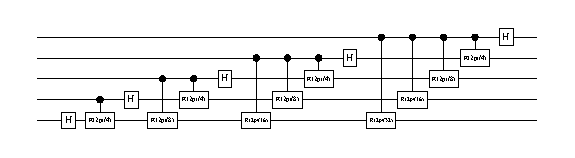
\includegraphics{qft}}
\]

  \caption{An implementation of the Quantum Fourier Transform on lists
    of qubits}
  \label{fig-qft}
\end{figure}


\section*{Glossary of Acronyms}
\addcontentsline{toc}{section}{Glossary of Acronyms}

\begin{itemize}
  \item QP = Proto-Quipper.
  \item QP' = Type-inference version of Proto-Quipper.
  \item QFT = Quantum Fourier Transform.
  \item QFT3 = Quantum Fourier Transform on three qubits.
  \item QLC = Quantum Lambda Calculus.
  \item USV = Unique Shortest Vector.
\end{itemize}

\bibliography{biblio}{}
\bibliographystyle{plain}
\addcontentsline{toc}{section}{Bibliography}

\end{document}

